\documentclass[11pt,a4paper, d]{scrartcl}
\usepackage{beamerarticle}
\usepackage[utf8]{inputenc}
\usepackage[T1]{fontenc}
\usepackage[english]{babel}
\usepackage[round]{natbib}
\usepackage{amsmath}
\usepackage{amsthm}
\usepackage{amssymb}
\usepackage{amsfonts}
\usepackage[scaled]{helvet}
\usepackage{amssymb}
\usepackage{multirow}
\usepackage{textcomp}
\usepackage{graphicx}
\usepackage{paralist}
\usepackage{textcomp}
\usepackage{pdflscape} 
\usepackage{marvosym}
\usepackage{pict2e}
\usepackage{float}
\usepackage{siunitx}
\usepackage[siunitx,european,cuteinductors,smartlabels]{circuitikz}
\usepackage{fancyhdr}
\usepackage{pgfplots}
\usepackage{sansmath}
\usetikzlibrary{shapes.geometric}
\usepackage{wasysym}
\usepackage{pdfpages}
\usepackage{fancyhdr}
\usepackage{hyperref}
\usepackage{thmtools}
%\usepackage{colorbrewer}
\usepackage{tabto,stackengine}
\usepgfplotslibrary{colorbrewer}
\usepgfplotslibrary{fillbetween}
\usetikzlibrary{graphs, automata, spy, positioning}
\usetikzlibrary{mindmap}
\usetikzlibrary{arrows}
\usepackage{subfig}
\usepackage{listings}
%\usepackage{ulem}

\usetikzlibrary{calc}

\graphicspath{{IntroDataScience/figures/}}
%\graphicspath{{../../figures/}}

\theoremstyle{definition}
%\declaretheorem{aufgabe}
\newtheorem{aufgabe}{Aufgabe}
%\definecolor{mint}{rgb}{32,178,170}
\DeclareMathOperator{\sign}{sgn}

\newcommand\MyBox[2]{
  \fbox{\lower0.75cm
    \vbox to 1.7cm{\vfil
      \hbox to 1.7cm{\hfil\parbox{1.4cm}{#1\\#2}\hfil}
      \vfil}%
  }%
}

\pgfmathdeclarefunction{norm}{3}{%
                      \pgfmathparse{sqrt(0.5*#3/pi)*exp(-0.5*#3*(#1-#2)^2)}%
                    }


\renewcommand*\familydefault{\sfdefault}
\renewcommand{\arraystretch}{1.1}

\pagestyle{fancy}
\fancyhf{}
\rhead{\begin{picture}(0,0)(0,0)\put(53,-62){
\includegraphics[height=4cm]{logoR}}\end{picture}}
\lhead{Handout - Introduction to Data Science}
\lfoot{File: \jobname, date: \today}
\rfoot{Page \thepage}

\author{Prof. Dr. Raphael Pfaff\\Lehrgebiet Schienenfahrzeugtechnik
\begin{picture}(0,0)(0,0)\put(158,390){
\includegraphics[height=4cm]{logoR}}\end{picture}}
\title{Rail Data Science}
\subtitle{Handout - Introduction to Data Science}
%\date{}


\begin{document}
\definecolor{mDarkBrown}{HTML}{604c38}
\definecolor{mDarkTeal}{HTML}{23373b}
\definecolor{mLightBrown}{HTML}{EB811B}
\definecolor{mLightGreen}{HTML}{14B03D}
\definecolor{mint}{RGB}{0,178,169}
\newcommand{\barP}{\, \mathrm{bar}}
\newcommand{\source}[1]{\rotatebox{90}{\tiny \color{gray} #1}}
\newcommand{\lehrtext}[1]{
\only<article>{
\vspace{0.3cm}
\leavevmode%
  \tabto*{-1.8cm}% LEFT MARGIN
  %\tabto*{\dimexpr\linewidth+40pt\relax}% RIGHT MARGIN
  \smash{\belowbaseline[-\ht\strutbox]{\makebox[0pt]%
%    [r]% LEFT MARGIN
    [l]% RIGHT MARGIN
  {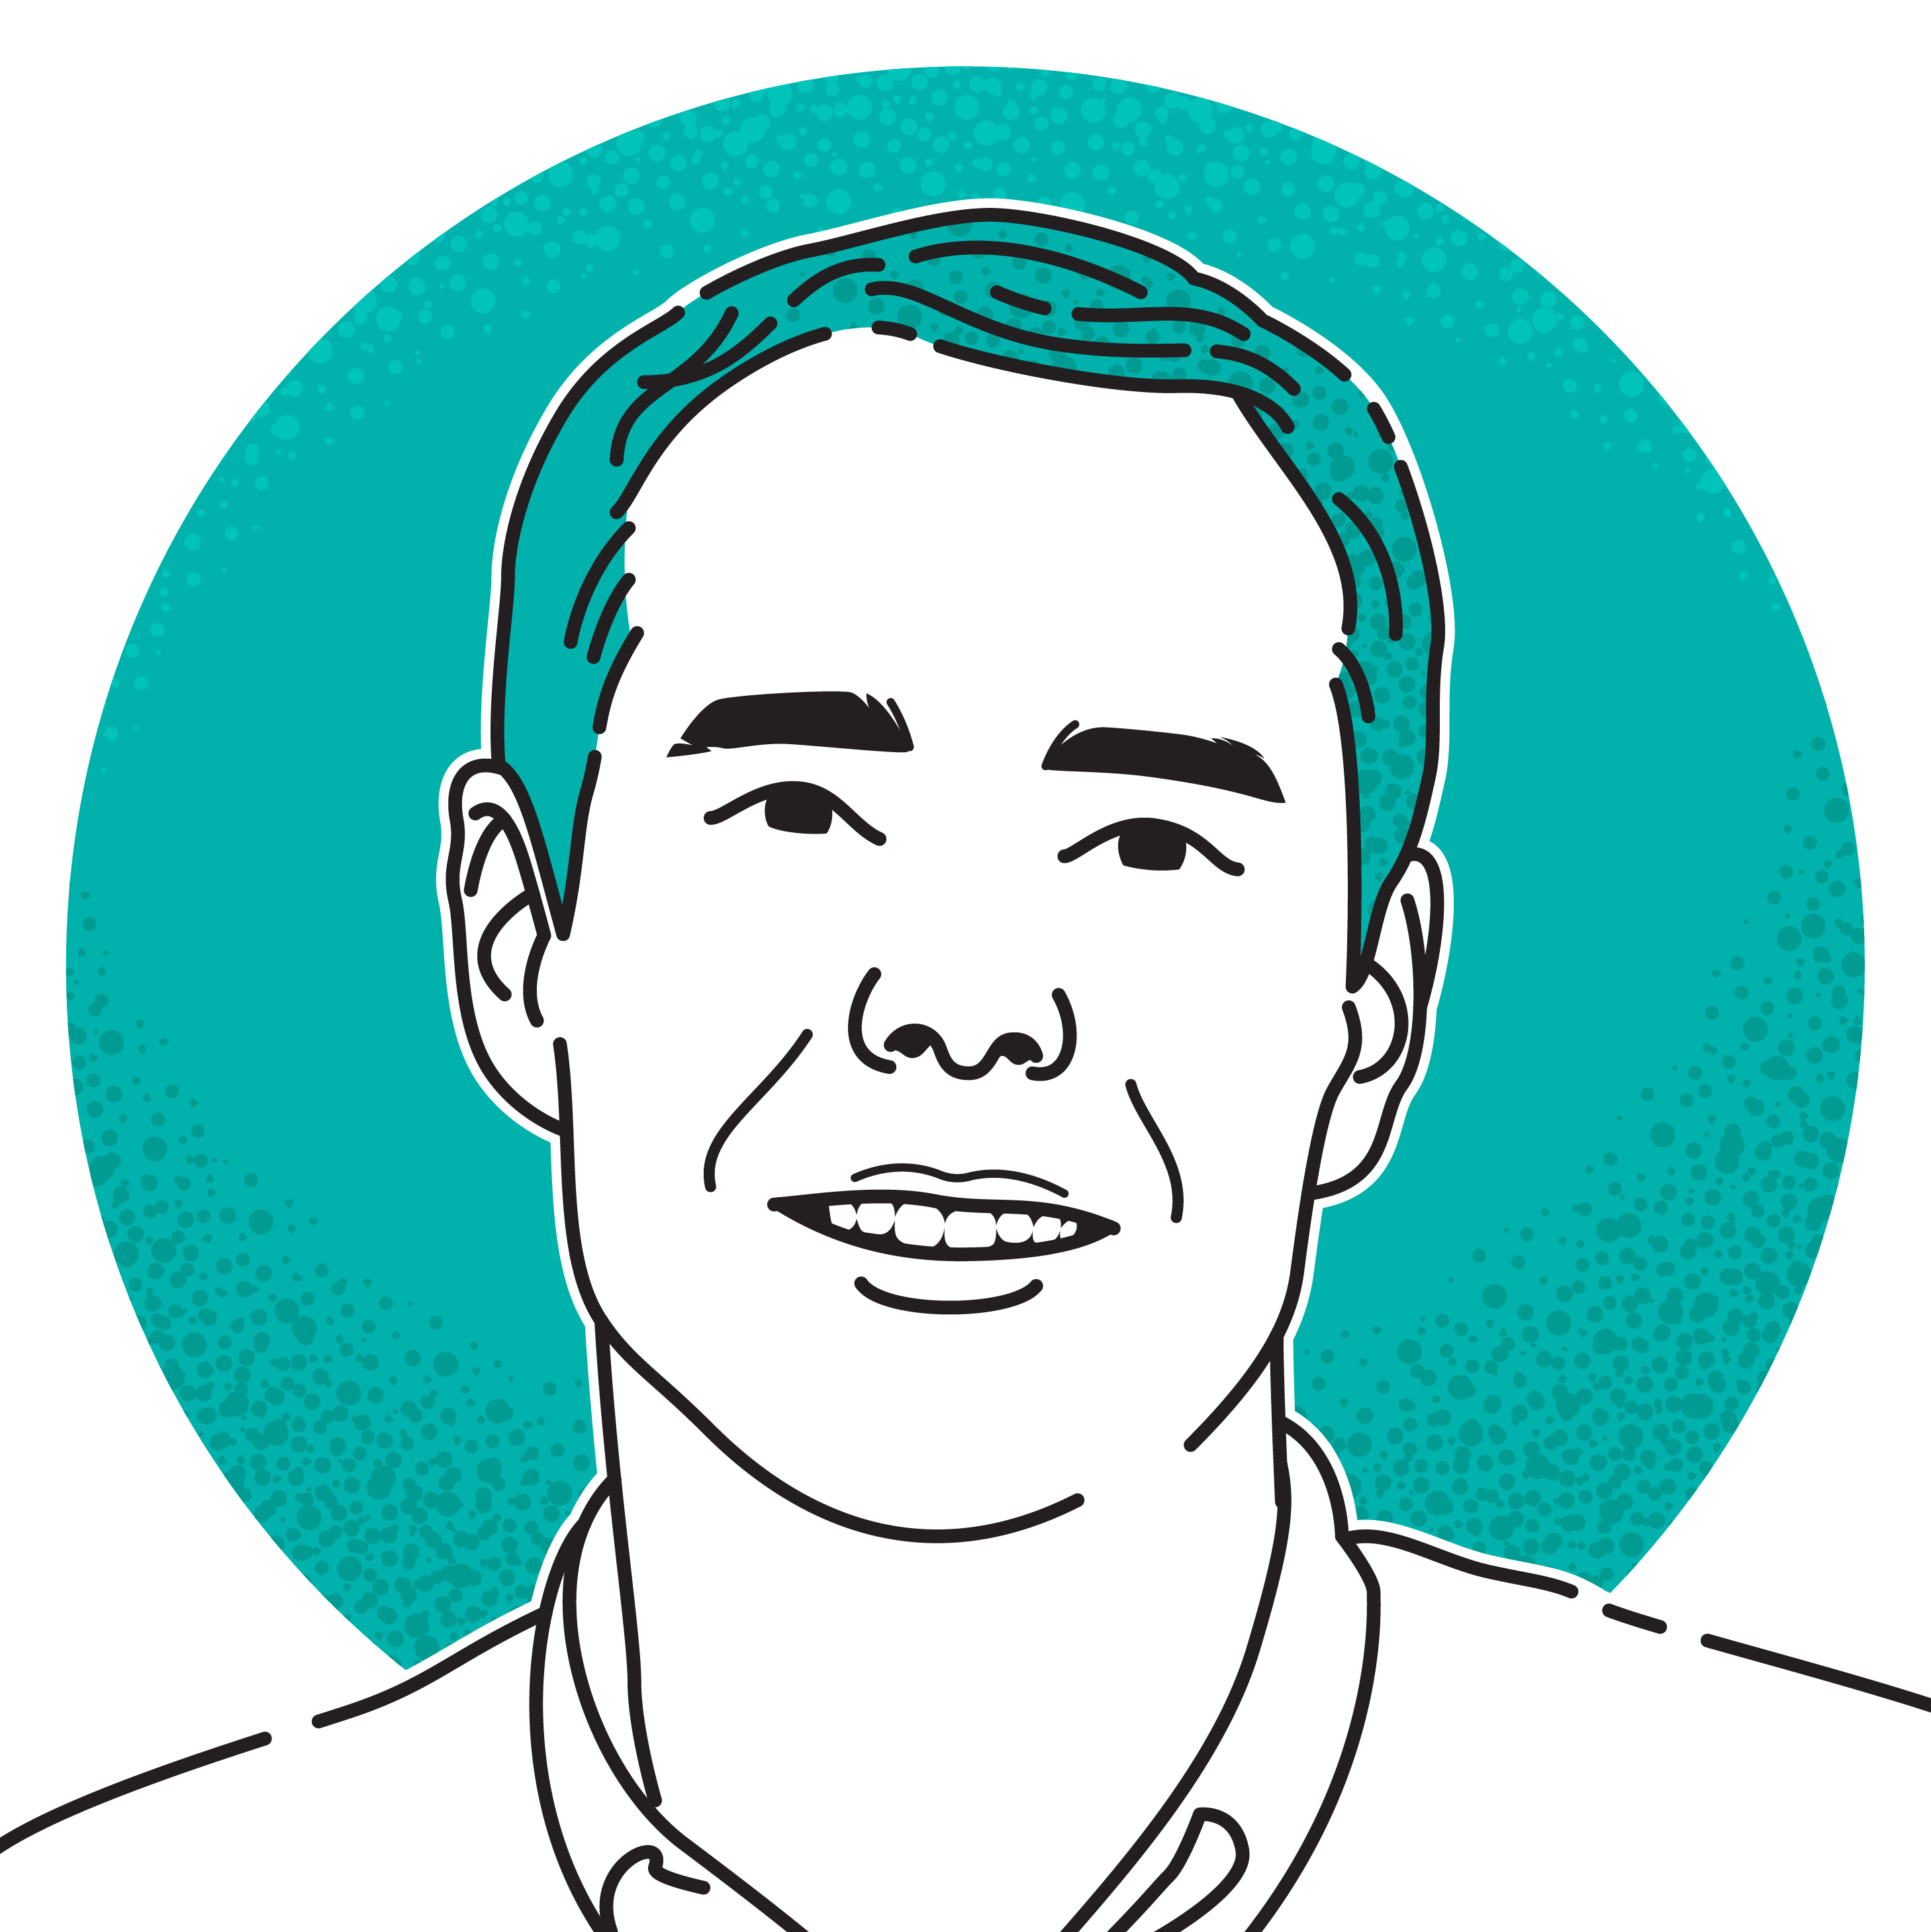
\includegraphics[width = 1.5cm]{teacher}}}}%
  \tabto*{\TabPrevPos}%
#1
}
}

\newcommand{\Var}{\operatorname{Var}}
\newcommand{\mum}{\operatorname{\mu m}}
\newcommand{\E}{\operatorname{E}}

\newcounter{exercise}
\newcommand*\theex{\stepcounter{exercise}\arabic{exercise}}

%\thispagestyle{fancy}
\maketitle
%\only<article>{
%\begin{tabular}{|c|p{10cm}|}
%\hline
%Datum & \"Anderung \\ \hline
%20.10.2020 & Erstausgabe \\ \hline
%28.12.2020 & Vervollständigung QM-Teil \\ \hline
%\end{tabular}
%}
%\newpage
%\tableofcontents
%%\newpage
%% \listoftheorems
%  \newpage
%%%%%%%%%%%%%%%%%%%%%
% 1. Pr\"aliminarien

\label{Sec:introDataScience}
%\subsection{Brief Introduction to Data Science}
\lehrtext{Data science as a field has far more applications than quality management, however quality management professionals take huge advantages from the application of data science tools and methods in their daily and non-daily work.

For this reason, enjoy this brief introduction and the more thorough hands-on training provided in the sequel!
}

\frame{\frametitle{What is Data Science?}
\lehrtext{Data science is our means of taming unstructured information and gathering insight. - Matthew Mayo, KDnuggets}
\begin{itemize}
\item Interdisciplinary field of
\begin{itemize}
		\item Systems,
		\item Methods and
		\item Processs to extract insight or knowledge from data.
\end{itemize}
\item Term coined in 2001, gained popularity in 2010
\item Integrates:
\begin{itemize}
		\item Data Engineering
		\item Scientific Method
		\item Mathematics
		\item Statistics
		\item Advanced Computational Methods
		\item Visualisation
		\item Hacker Mindset
		\item Domain Expertise
		\end{itemize}
\end{itemize}
}


\frame{\frametitle{How does Data Science integrate to Mechanical Engineering?}
\lehrtext{You may ask yourself: what is the point in learning to code in Python and apply data science tools, I am a mechanical engineer?

The short answer is: you will probably need it.

The longer answer is: your domain expertise, coupled with the willingness to dive into data, makes the difference!}

\begin{center}
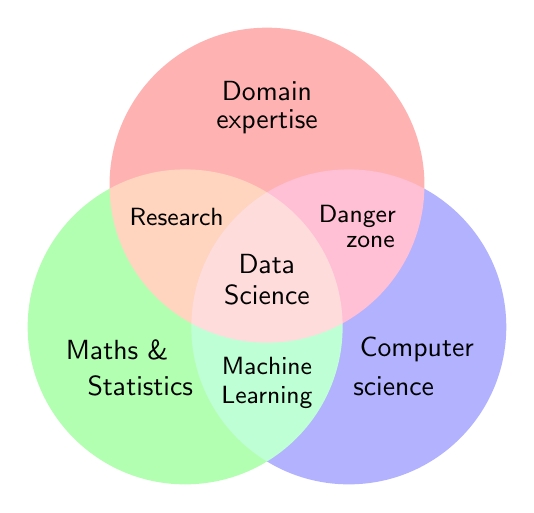
\begin{tikzpicture}
\begin{scope}[blend group=soft light]
\fill[red!30!white] ( 90:1.2) circle (2); 
\fill[green!30!white] (210:1.2) circle (2); 
\fill[blue!30!white] (330:1.2) circle (2); 
\end{scope}
%\node at ( 90:2.6) {Railway}; 
\node at ( 90:2.4) {Domain}; 
\node at ( 90:2.0) {expertise}; 
\node at (205:2.1) {Maths \&};
\node at (220:2.1) {Statistics}; 
\node at (335:2.1) {Computer}; 
\node at (320:2.1) {science}; 
%\node at (0,.4) {Rail};
\node at (0,0.2) {Data};
\node at (0,-.2) {Science};
\node at (270:1.1) {\small Machine};
\node at (270:1.5) {\small Learning};
\node at (145:1.4) {\small Research};
\node at (35:1.4) {\small Danger};
\node at (20:1.4) {\small zone};
\end{tikzpicture}
\end{center}
}

\frame{\frametitle{Why Data Sciene?}
\lehrtext{In a company context, you frequently act without proper information, although it is there - just nobody takes the time to analyse it. As soon as you show up to a board meeting or similar with data, people tend to trust your claims and you may be the one who is heard.

As Deming (the guy with the PDCA circle...) said:

\begin{quotation}
\textbf{In God we trust, all others bring data.}
\end{quotation}

Data science puts you in a position to:
}
\begin{columns}[t] 
     \begin{column}[T]{6cm} 
     	\begin{itemize}
     		\item Turn data to information
		\begin{itemize}
		\item Inform decisions
		\item Increase insight
		\end{itemize}
		\item Companies:
		\begin{itemize}
		\item Collect large amounts of data
		\item Do rarely integrate them
		\item Frequently decide based on the ``gut''
		\end{itemize}
     	\end{itemize}
     \end{column}
     	\begin{column}[T]{6cm} 
	\only<beamer>{
         	\begin{center}
            		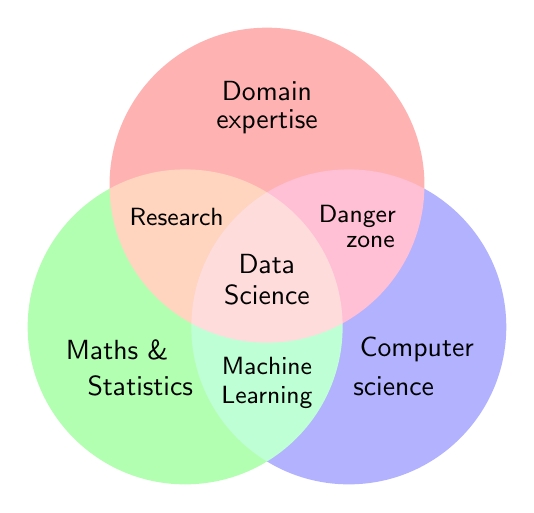
\begin{tikzpicture}
                            \begin{scope}[blend group=soft light]
                            \fill[red!30!white] ( 90:1.2) circle (2); 
                            \fill[green!30!white] (210:1.2) circle (2); 
                            \fill[blue!30!white] (330:1.2) circle (2); 
                            \end{scope}
                            %\node at ( 90:2.6) {Railway}; 
                            \node at ( 90:2.4) {Domain}; 
                            \node at ( 90:2.0) {expertise}; 
                            \node at (205:2.1) {Maths \&};
                            \node at (220:2.1) {Statistics}; 
                            \node at (335:2.1) {Computer}; 
                            \node at (320:2.1) {science}; 
                            %\node at (0,.4) {Rail};
                            \node at (0,0.2) {Data};
                            \node at (0,-.2) {Science};
                            \node at (270:1.1) {\small Machine};
                            \node at (270:1.5) {\small Learning};
                            \node at (145:1.4) {\small Research};
                            \node at (35:1.4) {\small Danger};
                            \node at (20:1.4) {\small zone};
                            \end{tikzpicture}

        		\end{center}}
     \end{column}
 \end{columns}
}

\frame{\frametitle{How do you increase Value with Data Science?}
\lehrtext{You are about to become engineers bearing the second highest education level in the EU (and world wide, for most countries) - perhaps you should bear in mind that the additional income and employer attractiveness come with some expectation: you are supposed to create value commensurate with your salary expectation and also your education level. Data Science may be helpful in this context.}
\begin{columns}[t] 
     \begin{column}[T]{6cm} 
     	\begin{itemize}
     		\item Improve decision making
		\begin{itemize}
		\item Empower management
		\item Supply data driven evidence
		\end{itemize}
		\item Identify trends and bring to action
		\item Challenge your colleagues
		\item Find opportunities for improvement
		\item Test decisions
		\item Understand customers
     	\end{itemize}
     \end{column}
     	\begin{column}[T]{6cm} 
	\only<beamer>{
         	\begin{center}
            		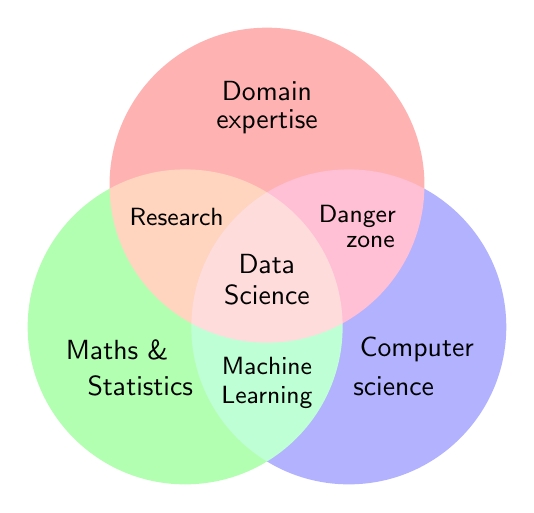
\begin{tikzpicture}
                            \begin{scope}[blend group=soft light]
                            \fill[red!30!white] ( 90:1.2) circle (2); 
                            \fill[green!30!white] (210:1.2) circle (2); 
                            \fill[blue!30!white] (330:1.2) circle (2); 
                            \end{scope}
                            %\node at ( 90:2.6) {Railway}; 
                            \node at ( 90:2.4) {Domain}; 
                            \node at ( 90:2.0) {expertise}; 
                            \node at (205:2.1) {Maths \&};
                            \node at (220:2.1) {Statistics}; 
                            \node at (335:2.1) {Computer}; 
                            \node at (320:2.1) {science}; 
                            %\node at (0,.4) {Rail};
                            \node at (0,0.2) {Data};
                            \node at (0,-.2) {Science};
                            \node at (270:1.1) {\small Machine};
                            \node at (270:1.5) {\small Learning};
                            \node at (145:1.4) {\small Research};
                            \node at (35:1.4) {\small Danger};
                            \node at (20:1.4) {\small zone};
                            \end{tikzpicture}

        		\end{center}}
     \end{column}
 \end{columns}
}

\frame{\frametitle{The data science process}
\lehrtext{The data science process starts with \emph{real world data}, which is messy, has missing values and all other ugly properties. So most of the time, you need to start with data cleaning and some exploration of the data set, mostly in the form of graphical analysis and looking at aggregated data.

As soon as you know something about your data, you are in a position to develop models and algorithms on your data set.

The result of both may be
\begin{enumerate}
\item a data product, e.g. a web app for data analysis or, more frequently in day-to-day work,
\item some form of communication, e.g. slides, a report, etc.,
\end{enumerate}
as displayed below:
}
         	\begin{center}
            		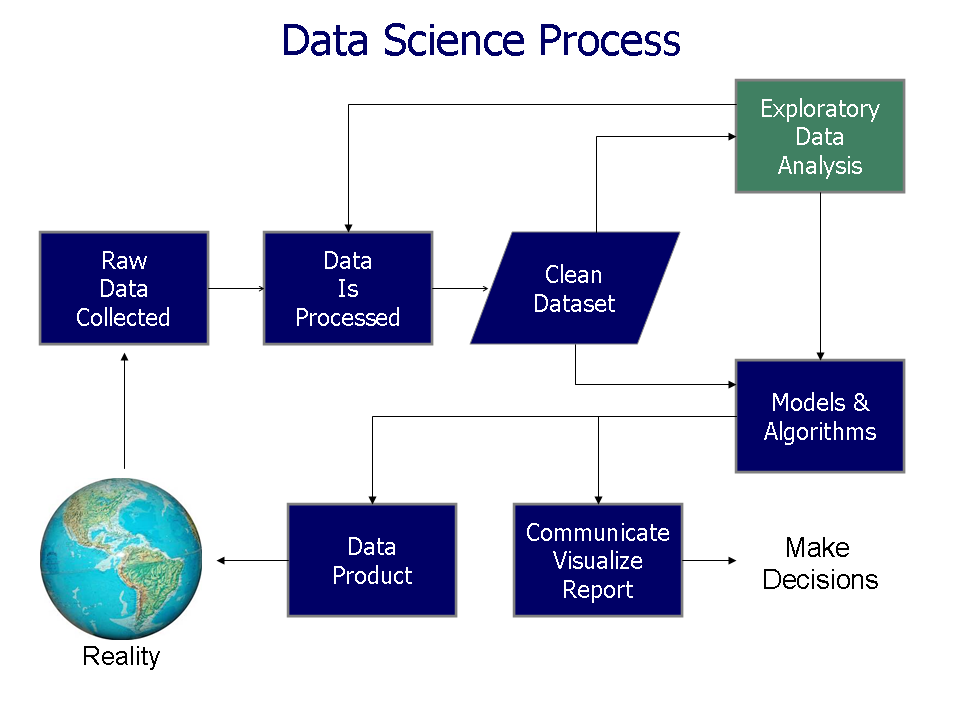
\includegraphics[width=0.7\textwidth]{DataScienceProcess}\source{Source: Farcaster/English Wikipedia}
        		\end{center}
   }

\frame{\frametitle{How to get started}
\lehrtext{In this module, we want you to get your hands \emph{dirty} on data, linked to quality-related problems. For this, you need some tools available locally. So, perhaps start early - mostly, installing anaconda is not a problem, sometimes however, it is made difficult by some system setups.

The actual steps will be subject of the more in-depth units to follow soon.}
\begin{itemize}
\item Set up your system. 
\begin{itemize}
		\item Install Anaconda to obtain Python/Jupyter
%		\item Set up a free education account with github.com
%		\item Install the app for your operating system
		\end{itemize}
\item Acquire data: start with popular open data sets. Get your company to make data accessible.
\item Ingest and transform: figure out the formats and sizes of your data. Find appropriate ways to import or access them.
\item Explore the data. Do you already find patterns from just plotting them?
\item Try your ``toolbox'' of methods (or a subset of it that sounds promising).
\item Visualise the results. Make your findings convincing to others: colleagues, managers, customers etc.
\end{itemize}
}
\newpage

\frame{\frametitle{Tools for Data Scientists}
\framesubtitle{}
\begin{columns}[t]
     \begin{column}[T]{6cm}
     	\begin{itemize}
     		\item Programming languages:
		\begin{itemize}
		\item R
		\item Python
		\item SAS
		\item ...
		\end{itemize}
		\item Visualisation app:
		\begin{itemize}
		\item Tableau
		\end{itemize}
		\item Development Environment (IDE):
		\begin{itemize}
		\item Jupyter
		\item Spyder
		\end{itemize}
		\item Also potentially:
		\begin{itemize}
		\item Matlab
		\item Scilab
		\item ...
		\end{itemize}
     	\end{itemize}
     \end{column}
     	\begin{column}[T]{6cm}
         	\begin{center}
            		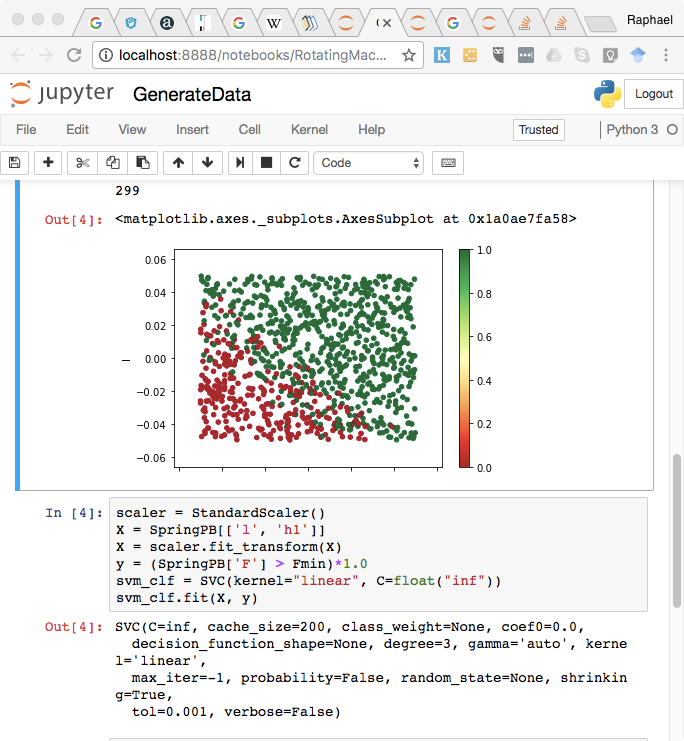
\includegraphics[width=6cm]{Jupyter}\source{}
            		\\ 
		
		{\scriptsize For installation, visit: \url{https://www.anaconda.com/products/individual}{https://www.anaconda.com/products/individual}}
        		\end{center}
     \end{column}
 \end{columns}
}

\frame{\frametitle{Selected Techniques applied in Data Science}
\framesubtitle{}
{\only<beamer>{\footnotesize}
\begin{itemize}
\item \textbf{Visualisation}
\item Regression: Linear, Logistic
\item \textbf{Density Estimation}
\item Confidence Intervals
\item Test of Hypotheses
\item Pattern Recognition
\item {Time Series}
\item \textbf{Unsupervised Learning (Clustering)}
\item Supervised Learning
\item Decision Trees
\item \textbf{Monte-Carlo-Simulation}
\item Bayesian Statistics
\item Principal Component Analysis
\item \textbf{Support Vector Machines}
\end{itemize}
}
}

%\input{parts/part2}
%% !TEX root = ../MdQM-Folien.tex
\section{Data Science: Tools and Techniques}
\frame{\frametitle{Tools for Data Scientists}
\framesubtitle{}
\begin{columns}[t]
     \begin{column}[T]{6cm}
     	\begin{itemize}
     		\item Programming languages:
		\begin{itemize}
		\item R
		\item Python
		\item SAS
		\item ...
		\end{itemize}
		\item Visualisation app:
		\begin{itemize}
		\item Tableau
		\end{itemize}
		\item Development Environment (IDE):
		\begin{itemize}
		\item Jupyter
		\item Spyder
		\end{itemize}
		\item Also potentially:
		\begin{itemize}
		\item Matlab
		\item Scilab
		\item ...
		\end{itemize}
     	\end{itemize}
     \end{column}
     	\begin{column}[T]{6cm}
         	\begin{center}
            		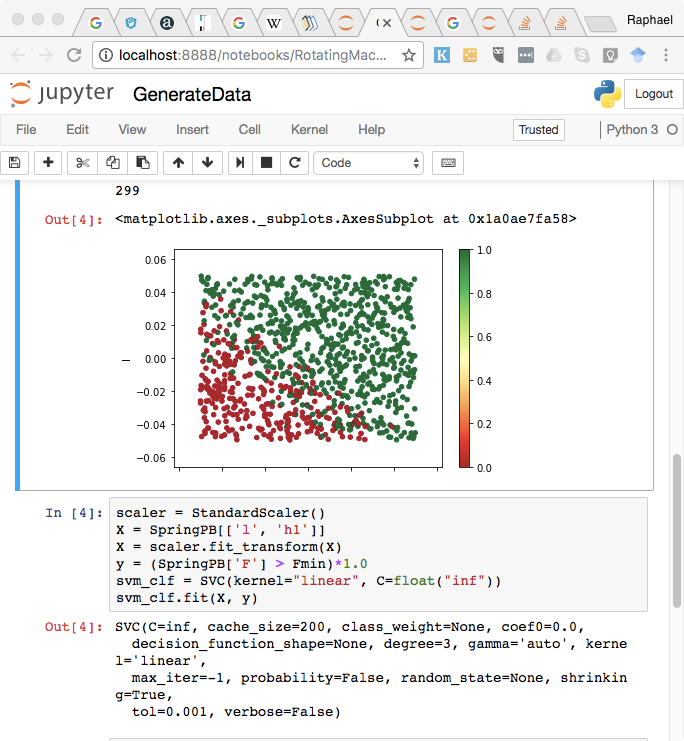
\includegraphics[width=0.85\textwidth]{Jupyter}\source{}
            		\\ {\scriptsize For installation, visit: http://jupyter.org/install.html}
        		\end{center}
     \end{column}
 \end{columns}
}

\frame{\frametitle{Selected Techniques applied in Data Science}
\framesubtitle{}
{\footnotesize
\begin{itemize}
\item \textbf{Visualisation}
\item Regression: Linear, Logistic
\item \textbf{Density Estimation}
\item Confidence Intervals
\item Test of Hypotheses
\item Pattern Recognition
\item {Time Series}
\item Unsupervised Learning (Clustering)
\item Supervised Learning
\item Decision Trees
\item \textbf{Monte-Carlo-Simulation}
\item Bayesian Statistics
\item \textbf{Principal Component Analysis}
\item \textbf{Support Vector Machines}
\end{itemize}
}
}

\frame{\frametitle{Visualisation approaches}
\lehrtext{There are a multitude of visualisation approaches, here we present you with some so that you extend your toolbox beyond the standard column, cake and line diagram omnipresent in MS Excel analyses.}
\begin{columns}[t]
     \begin{column}[T]{6cm}
     	\only<beamer>{\begin{itemize}
     	\item \textbf{Line plot with / w/o confidence}
		\item Bar plots (stacked/grouped)
		\item Histogram
		\item Scatter plot
		\begin{itemize}
		\item Blob type
		\item Colors
		\end{itemize}
		\item Box whisker
		\item Bubble chart
		\item Geospatial plots
		\item Surface plot
		\item Heat map
     	\end{itemize}}
	\only<article>{\vspace{1cm}}
	\lehrtext{ 
	\begin{itemize}
     	\item Line plot with / w/o confidence: these give an idea of continuous developments, in the example below the development of model misfit over model order. A confidence interval yields additional insight if repeated experiments are the basis of each data point.
		\item Bar plots (stacked/grouped): the stacked bar plots shown below illustrate at the same time relative and absolute data, in the case at hand market sizes and distributions.
		\item Histogram: useful to show the distribution of a parameter.
		\item Scatter plot: useful if two or three variables with 2 continuous value ranges and a third class or variable property of the data point, displayed as:
		\begin{itemize}
		\item Blob type
		\item Colors
		\end{itemize}
		\item Box whisker: very useful to show distribution data, e.g. mean, standard deviation and min/max values.
		\item Bubble chart: alternative to bar charts for display of relative and absolute data in one chart.
		\item Geospatial plots: useful (and necessary for data that indicates locations of data. The example shows power usage on a railway line.
		\item Surface plot: very technical display of 3D data.
		\item Heat map: color coded version of 3D data with regularly spaced $x$ and $y$ intervals.
     	\end{itemize}
	}
     \end{column}
     \begin{column}[T]{6cm}
       	\begin{center}
				\begin{figure}[htbp]
					\centering
					\includegraphics[width=6cm]{lineplot}
					\caption{Example line plot}
				\end{figure}
\only<article>{
				\begin{figure}[htbp]
					\centering
					\includegraphics[width=6cm]{barplot}
					\caption{Example bar plot}
				\end{figure}
				
				\begin{figure}[htbp]
					\centering
					\includegraphics[width=6cm]{histogram}
					\caption{Example histogram}
				\end{figure}
				
				\begin{figure}[htbp]
					\centering
					\includegraphics[width=6cm]{scatterplot}
					\caption{Example scatter plot}
				\end{figure}
				
				\begin{figure}[htbp]
					\centering
					\includegraphics[width=6cm]{boxplot}
					\caption{Example box whisker plot}
				\end{figure}
				
				\begin{figure}[htbp]
					\centering
					\includegraphics[width=6cm]{bubblechart}
					\caption{Example bubble chart}
				\end{figure}
				
				\begin{figure}[htbp]
					\centering
					\includegraphics[width=6cm]{geospatialplot}
					\caption{Example geospatial plot}
				\end{figure}
				
				\begin{figure}[htbp]
					\centering
					\includegraphics[width=6cm]{surfaceplot}
					\caption{Example surface plot}
				\end{figure}
				
				\begin{figure}[htbp]
					\centering
					\includegraphics[width=6cm]{heatmap}
					\caption{Example heatmap}
				\end{figure}
				
}
%				{\tiny Beispiel}
     	\end{center}
     \end{column}
 \end{columns}
}

\only<beamer>{\frame{\frametitle{Visualisation approaches}
\begin{columns}[t]
     \begin{column}[T]{6cm}
     	\begin{itemize}
     	\item Line plot with / w/o confidence
		\item \textbf{Bar plots (stacked/grouped)}
		\item Histogram
		\item Scatter plot
		\begin{itemize}
		\item Blob type
		\item Colors
		\end{itemize}
		\item Box whisker
		\item Bubble chart
		\item Geospatial plots
		\item Surface plot
		\item Heat map
     	\end{itemize}
     \end{column}
     \begin{column}[T]{6cm}
       	\begin{center}
				\begin{figure}[h]
					\centering
					\includegraphics[width=.85\linewidth]{barplot}
				\end{figure}
     	\end{center}
     \end{column}
 \end{columns}
}

\frame{\frametitle{Visualisation approaches}
\begin{columns}[t]
     \begin{column}[T]{6cm}
     	\begin{itemize}
     	\item Line plot with / w/o confidence
		\item Bar plots (stacked/grouped)
		\item \textbf{Histogram}
		\item Scatter plot
		\begin{itemize}
		\item Blob type
		\item Colors
		\end{itemize}
		\item Box whisker
		\item Bubble chart
		\item Geospatial plots
		\item Surface plot
		\item Heat map
     	\end{itemize}
     \end{column}
     \begin{column}[T]{6cm}
       	\begin{center}
				\begin{figure}[h]
					\centering
					\includegraphics[width=.95\linewidth]{histogram}
				\end{figure}
     	\end{center}
     \end{column}
 \end{columns}
}

\frame{\frametitle{Visualisation approaches}
\begin{columns}[t]
     \begin{column}[T]{6cm}
     	\begin{itemize}
     	\item Line plot with / w/o confidence
		\item Bar plots (stacked/grouped)
		\item Histogram
		\item \textbf{Scatter plot}
		\begin{itemize}
		\item Blob type
		\item Colors
		\end{itemize}
		\item Box whisker
		\item Bubble chart
		\item Geospatial plots
		\item Surface plot
		\item Heat map
     	\end{itemize}
     \end{column}
     \begin{column}[T]{6cm}
       	\begin{center}
				\begin{figure}[h]
					\centering
					\includegraphics[width=.95\linewidth]{scatterplot}
				\end{figure}
     	\end{center}
     \end{column}
 \end{columns}
}

\frame{\frametitle{Visualisation approaches}
\begin{columns}[t]
     \begin{column}[T]{6cm}
     	\begin{itemize}
     	\item Line plot with / w/o confidence
		\item Bar plots (stacked/grouped)
		\item Histogram
		\item Scatter plot
		\begin{itemize}
		\item Blob type
		\item Colors
		\end{itemize}
		\item \textbf{Box whisker}
		\item Bubble chart
		\item Geospatial plots
		\item Surface plot
		\item Heat map
     	\end{itemize}
     \end{column}
     \begin{column}[T]{6cm}
       	\begin{center}
				\begin{figure}[h]
					\centering
					\includegraphics[width=.95\linewidth]{boxplot}
				\end{figure}
     	\end{center}
     \end{column}
 \end{columns}
}

\frame{\frametitle{Visualisation approaches}
\begin{columns}[t]
     \begin{column}[T]{6cm}
     	\begin{itemize}
     	\item Line plot with / w/o confidence
		\item Bar plots (stacked/grouped)
		\item Histogram
		\item Scatter plot
		\begin{itemize}
		\item Blob type
		\item Colors
		\end{itemize}
		\item Box whisker
		\item \textbf{Bubble chart}
		\item Geospatial plots
		\item Surface plot
		\item Heat map
     	\end{itemize}
     \end{column}
     \begin{column}[T]{6cm}
       	\begin{center}
				\begin{figure}[h]
					\centering
					\includegraphics[width=.95\linewidth]{bubblechart}
				\end{figure}
     	\end{center}
     \end{column}
 \end{columns}
}

\frame{\frametitle{Visualisation approaches}
\begin{columns}[t]
     \begin{column}[T]{6cm}
     	\begin{itemize}
     	\item Line plot with / w/o confidence
		\item Bar plots (stacked/grouped)
		\item Histogram
		\item Scatter plot
		\begin{itemize}
		\item Blob type
		\item Colors
		\end{itemize}
		\item Box whisker
		\item Bubble chart
		\item \textbf{Geospatial plots}
		\item Surface plot
		\item Heat map
     	\end{itemize}
     \end{column}
     \begin{column}[T]{6cm}
       	\begin{center}
				\begin{figure}[h]
					\centering
					\includegraphics[width=.95\linewidth]{geospatialplot}
				\end{figure}
     	\end{center}
     \end{column}
 \end{columns}
}

\frame{\frametitle{Visualisation approaches}
\begin{columns}[t]
     \begin{column}[T]{6cm}
     	\begin{itemize}
     	\item Line plot with / w/o confidence
		\item Bar plots (stacked/grouped)
		\item Histogram
		\item Scatter plot
		\begin{itemize}
		\item Blob type
		\item Colors
		\end{itemize}
		\item Box whisker
		\item Bubble chart
		\item Geospatial plots
		\item \textbf{Surface plot}
		\item Heat map
     	\end{itemize}
     \end{column}
     \begin{column}[T]{6cm}
       	\begin{center}
				\begin{figure}[h]
					\centering
					\includegraphics[width=.95\linewidth]{surfaceplot}
				\end{figure}
     	\end{center}
     \end{column}
 \end{columns}
}

\frame{\frametitle{Visualisation approaches}
\begin{columns}[t]
     \begin{column}[T]{6cm}
     	\begin{itemize}
     	\item Line plot with / w/o confidence
		\item Bar plots (stacked/grouped)
		\item Histogram
		\item Scatter plot
		\begin{itemize}
		\item Blob type
		\item Colors
		\end{itemize}
		\item Box whisker
		\item Bubble chart
		\item Geospatial plots
		\item Surface plot
		\item \textbf{Heat map}
     	\end{itemize}
     \end{column}
     \begin{column}[T]{6cm}
       	\begin{center}
				\begin{figure}[h]
					\centering
					\includegraphics[width=1.0\linewidth]{heatmap}
				\end{figure}
     	\end{center}
     \end{column}
 \end{columns}
}}

\subsection{Density Estimation}
\frame{\frametitle{Density estimation}
\lehrtext{Estimate underlying probability density function from observed data, which is often required in a production context to describe what is likely to happen in the future.}
\begin{columns}[t]
     \begin{column}[T]{6cm}
     	\begin{itemize}
     		\item Analysis of distribution properties from sampled data
		\item Fit an appropriate kernel to the samples
     	\end{itemize}
     \end{column}
     	\begin{column}[T]{6cm}
         	\begin{center}
		\pgfplotsset{compat=newest,
                      tick label style={font=\sansmath\sffamily},
                      axis line style={draw=black!80, line width=0.1875ex},
                      y tick label style={/pgf/number format/fixed},
                      tick style={major tick length=0.0ex},
                      major grid style={thick, dash pattern=on 0pt off 2pt, black!50},
                      height = 6cm
                    }

            		\begin{tikzpicture}[line cap=round, line join=round]
                    \begin{axis}[ymajorgrids, xmajorgrids]
                    \addplot [ybar, domain=0:15, samples=16, fill=blue!50!cyan, draw=none]
                      (x, {0.6*norm(x, 4, 0.1) + 0.4*norm(x, 12, .05)});
                    \addplot [very thick, draw=orange,  domain=0:15, samples=100, smooth]
                      (x, {0.6*norm(x, 4, 0.1) + 0.4*norm(x, 12, .05) });
                    \end{axis}
                    \end{tikzpicture}
        		\end{center}
     \end{column}
 \end{columns}
}
%\subsubsection{Time Series}
\newpage
\subsection{Machine Learning concept}


\frame{\frametitle{What is machine learning?}
\lehrtext{ML is a field of study that gives computers the ability to learn without being explicitly programmed.}
\begin{columns}[t]
     \begin{column}[T]{7cm}
     	\begin{itemize}
     		\item Different paradigm:
		\begin{itemize}
		\item Derive rules from observations
		\end{itemize}
		\item Typical procedure:
		\begin{itemize}
		\item \textbf{Train:} Observe set of examples ``training data''
		\item \textbf{Fit:} Infer information of process behind data
		\item \textbf{Test:} Make prediction on unseen data ``Test data''
		\end{itemize}
		\item Variations:
		\begin{itemize}
		\item Supervised learning: provide labels with data
		\item Unsupervised learning: cluster data based on patterns
		\end{itemize}
     	\end{itemize}
     \end{column}
     	\begin{column}[T]{7cm}
         	\begin{center}
			Traditional approach:
			\vspace{.5cm}
			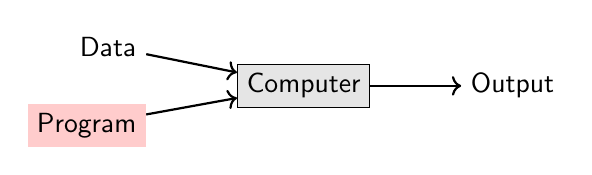
\begin{tikzpicture}
 				\node[anchor = east] (d) at (0,0) {Data};
				\node[anchor = east, fill = red!20] (p) at (0,-1) {Program};
				\node[anchor = west] (o) at (4,-.5) {Output};
				\node[draw, fill = gray!20] (c) at (2,-.5) {Computer};
				\draw[->, thick] (d) -- (c);
				\draw[->, thick] (p)-- (c);
				\draw[->, thick] (c) -- (o);
			\end{tikzpicture}

			Machine learning approach:
			\vspace{.5cm}
			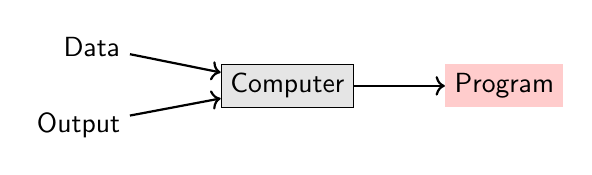
\begin{tikzpicture}
 				\node[anchor = east] (d) at (0,0) {Data};
				\node[anchor = east] (p) at (0,-1) {Output};
				\node[anchor = west,  fill = red!20] (o) at (4,-.5) {Program};
				\node[draw, fill = gray!20] (c) at (2,-.5) {Computer};
				\draw[->, thick] (d) -- (c);
				\draw[->, thick] (p)-- (c);
				\draw[->, thick] (c) -- (o);
			\end{tikzpicture}

		\end{center}
     \end{column}
 \end{columns}
}

\subsubsection{Unsupervised Learning (Clustering)}
\frame{\frametitle{Clustering}
\framesubtitle{Two fundamental approaches, $k$ number of clusters defined \textit{a priori}}
\begin{columns}[t]
     \begin{column}[T]{7cm}
     \textbf{Hierarchical clustering}
     	\begin{enumerate}
     		\item Assign each item to one cluster
		\item Find closest (most similar cluster): merge them
		\item Continue until desired number of clusters $k$ is reached
     	\end{enumerate}
     \end{column}
     	\begin{column}[T]{7cm}
         	\textbf{K-means clustering}
     	\begin{enumerate}
		\item Randomly choose $k$ initial centroids
		\item While centroids don't change
		\begin{enumerate}
		\item[E:] Create $k$ clusters by assigning each item to closest centroid
		\item[M:] Compute $k$ new centroids by averaging items in each cluster
		\end{enumerate}
     	\end{enumerate}
     \end{column}
 \end{columns}

\begin{center}
 	\includegraphics[width = .9\textwidth]{expectation-maximization}
\end{center}
}

\frame{\frametitle{K-means clustering procedure}
         	\begin{center}
            		\only<1>{\includegraphics[width=0.7\textwidth]{PCAprocedure0}\source{}}
			\only<2>{\includegraphics[width=0.7\textwidth]{PCAprocedure1}\source{}}
			\only<3>{\includegraphics[width=0.7\textwidth]{PCAprocedure2}\source{}}
			\only<4>{\includegraphics[width=0.7\textwidth]{PCAprocedure3}\source{}}
			\only<5>{\includegraphics[width=0.7\textwidth]{PCAprocedure4}\source{}}
			\only<6>{\includegraphics[width=0.7\textwidth]{PCAprocedure5}\source{}}
			%\only<7>{\includegraphics[width=0.7\textwidth]{PCAprocedure6}\source{}}

        		\end{center}}

\frame{\frametitle{K-means inappropriate cluster number}
         	\begin{center}
            		\only<1>{\includegraphics[width=0.7\textwidth]{PCAprocedureFewCluster0}\source{}}
			\only<2>{\includegraphics[width=0.7\textwidth]{PCAprocedureFewCluster1}\source{}}
			\only<3>{\includegraphics[width=0.7\textwidth]{PCAprocedureFewCluster2}\source{}}
			\only<4>{\includegraphics[width=0.7\textwidth]{PCAprocedureFewCluster3}\source{}}
			\only<5>{\includegraphics[width=0.7\textwidth]{PCAprocedureFewCluster4}\source{}}
			\only<6>{\includegraphics[width=0.7\textwidth]{PCAprocedureFewCluster5}\source{}}
			%\only<7>{\includegraphics[width=0.7\textwidth]{PCAprocedure6}\source{}}

        		\end{center}}

\subsubsection{Monte-Carlo-Simulation}
\frame{\frametitle{Monte-Carlo-Simulation (MC-Simulation) recap}
\framesubtitle{}
\begin{itemize}
\item Method of estimating value of unknown quantity using inferential statistics
\item Inferential statistics terms:
\begin{itemize}
		\item Population: set of examples
		\item Sample: Proper subset of population
\end{itemize}
\item Random sample tends to exhibit same properties as population it is drawn from
\end{itemize}
\begin{example}[Flip coins]
 Let's estimate the probabilities of heads vs. tails for an infinite number of coin flips:
 \begin{itemize}
		\item One flip (heads): 100\% heads?
		\item Two flips (h, h): still 100 \% heads? Confidence level?
		\item 100 flips (52 h, 48 t): Probability of next coin coming up heads 52/100.
		\end{itemize}
\end{example}
}

\frame{\frametitle{Key aspects to be asked in MC-Simulations}
\framesubtitle{}
\begin{itemize}
\item Never possible to guarantee perfect accuracy through sampling
\item Never assume that an estimate is precisely correct
\item How many samples do we need to look at before we can have justified confidence in our answers?
\begin{itemize}
	\item Answer depends on underlying distribution
	\item Especially hard for defects ``Rare event simulation''
\end{itemize}
\end{itemize}
}

\subsubsection{Monte-Carlo-Simulation Application Example}
\frame{\frametitle{MC-Simulation application example: Braking curve}
\framesubtitle{CCS systems rely on braking curves to describe the train's braking capability.}
\begin{columns}[t]
     \begin{column}[T]{6cm}
     	\begin{itemize}
     		\item To supervise train velocity, CCS systems predict the future braking capability of the train
		\item However, there is not \textit{the} braking capability
		\item Braking curves exhibit a randomised behaviour
     	\end{itemize}
     \end{column}
     	\begin{column}[T]{6cm}
         	\begin{center}
			\includegraphics[width=\textwidth]{brakingcurvesND}
        		\end{center}
     \end{column}
 \end{columns}
}

\frame{\frametitle{White Box Modelling of the braking system}
\framesubtitle{Which parameters can be identified and which effect do they have on the braking distance?}
\begin{itemize}
\item Brake pipe: propagation velocity, flow resistances, train length
\item Distributor valve: Filling time, brake cylinder pressure
\item Braking force generation: efficiency, brake radius (for disc brakes), pad/block friction coefficient
\item Wheel/rail contact: rail surface, contaminants, slip, ...
\end{itemize}
\begin{center}
\begin{center}
          \includegraphics[width=\textwidth]{TrainBPDiagram}
\end{center}
\end{center}
\begin{itemize}
	\item Also discrete failure events need to be considered
\end{itemize}
}



\frame{\frametitle{Why chose MC-Simulation? What are the challenges?}
\framesubtitle{}
\begin{itemize}
\item Error-propagation:
\begin{itemize}
		\item Conservative: assumes normal distribution for all parameters
		\item Complex: requires explicit function formulation and partial differentiation
\end{itemize}
\item (Standard) Monte-Carlo-Simulation:
\begin{itemize}
		\item Efficient (in terms of confidence): returns shortest (also asymmetric) confidence interval
		\item Inefficient (in terms of computational effort):
		\begin{itemize}
		\item For rare event $\varepsilon \ll 1$, $N \approx \frac{100}{\varepsilon}$ trials required
		\item Typical according to CSM: $\varepsilon \in \left[10^{-7} \ldots  10^{-9}\right] \, \Rightarrow \, N \approx 10^{11}$
		\end{itemize}
\end{itemize}
\item ERA proposes to precalculate braking curves for limited number of train formations
\begin{itemize}
		\item Freight trains to be handled using braked weight and correction factor
		\end{itemize}
\end{itemize}
}

\frame{\frametitle{Importance sampling for MC-Simulations}
\framesubtitle{Importance sampling (IS) increases the probability of ``desired'' outcomes in Monte-Carlo-Simulations.}
\begin{itemize}
\item Typical IS approaches:
\begin{itemize}
		\item Stratification: select only relevant strata of the sampling range
		\item Scaling: Scale random variable
		\item Translation: Move random variable to more relevant part of sampling space
		\item Change of random variable: Replace random variable by one more likely to produce outcomes in the relevant range
		\item Adaptive approaches
		\end{itemize}
\item Effect: higher number of samples in region of interest
\item Correction factor: Likelihood ratio $L(y) = \frac{f(y)}{\tilde{f}(y)}$
\end{itemize}
}

\frame{\frametitle{Application of IS to braking curves}
\framesubtitle{Select relevant variables for IS.}
\begin{center}
\includegraphics[width = .8\textwidth]{mhist}
\end{center}
}

\frame{\frametitle{Application of IS to braking curves}
\framesubtitle{Change identified random variables, in the case at hand $\mu_{B}$}
\begin{center}
\includegraphics[width = .8\textwidth]{BChist}
\end{center}
}

\frame{\frametitle{Application of IS to braking curves}
\framesubtitle{Analyse for rare events, here braking distances in excess of 1100 m. $N = 5 \cdot 10^7$}
\only<1>{\begin{center}
\includegraphics[width = .8\textwidth]{rare}
\end{center}}
\only<2>{
\begin{center}
%\hspace{-.62cm}
\begin{tabular}{|c|c|c|c|c|c|c|}
\hline
$s$ & $n_{\mathcal{U}}$ & $p_{\mathcal{U}}$ & $n_{IS, 1}$ & $p_{IS, 1}$ & $n_{IS, 2}$ & $p_{IS, 2}$ \\ \hline
1000 & 24400 & 4.89$\cdot 10^{-3}$ & 2.27$\cdot 10^6$ & 1.14$\cdot 10^{-2}$ & 3.11$\cdot 10^5$ & 1.77$\cdot 10^{-3}$ \\ \hline
1050 & 2 & 4$\cdot 10^{-7}$ & 6.66$\cdot 10^4$ & 2.02$\cdot 10^{-4}$ & 1.48$\cdot 10^4$ & 1.59$\cdot 10^{-4}$ \\ \hline
1100 & 0 & 0 & 115 & 2.04$\cdot 10^{-7}$ & 419 & 7.50$\cdot 10^{-6}$ \\ \hline
1150 & 0 & 0 & 0 & 0 & 15 & 3.88$\cdot 10^{-7}$ \\ \hline
1160 & 0 & 0 & 0 & 0 & 7 & 2.05$\cdot 10^{-7}$ \\ \hline
1170 & 0 & 0 & 0 & 0 & 5 & 1.46$\cdot 10^{-7}$ \\ \hline
1180 & 0 & 0 & 0 & 0 & 4 & 1.16$\cdot 10^{-7}$ \\ \hline
1190 & 0 & 0 & 0 & 0 & 1 & 2.90$\cdot 10^{-8}$ \\ \hline
\end{tabular}
\end{center}
}
}



\subsection{Principal Component Analysis}
\frame{\frametitle{Principal Component Analysis}

Principle Component Analysis (PCA) = Hauptkomponentenanalyse

\begin{itemize}
\setlength{\itemsep}{10pt}
\item Verfahren der multivariaten Statistik, parallele Untersuchung mehrerer statistischer Variablen auf deren Abh"angigkeiten
\item 1901 von Karl Pearson eingef"uhr, in den 1930er Jahren von Harold Hotelling weiterentwickelt
\item Un"uberwachtes Lernen; keine Trainingsdaten, keine Belohngsfunktion
\end{itemize}

}







%%%%%%%%%%%%%%%%%%%%%%%%%%%%%%%%%%%
%%%      PCA - Geometrisch      %%%
%%%%%%%%%%%%%%%%%%%%%%%%%%%%%%%%%%%

\begin{frame}

\frametitle{PCA -- Geometrisch}

\begin{figure}[h]
\centering
\includegraphics[width=.65\linewidth]{pca_images/pca_zweidimensional_0}
\end{figure}

\end{frame}






%%%%%%%%%%%%%%%%%%%%%%%%%%%%%%%%%%%
%%%      PCA - Geometrisch      %%%
%%%%%%%%%%%%%%%%%%%%%%%%%%%%%%%%%%%

\begin{frame}

\frametitle{PCA -- Geometrisch}

\begin{figure}[h]
\centering
\includegraphics[width=.65\linewidth]{pca_images/pca_zweidimensional_1}
\end{figure}

\end{frame}






%%%%%%%%%%%%%%%%%%%%%%%%%%%%%%%%%%%
%%%      PCA - Geometrisch      %%%
%%%%%%%%%%%%%%%%%%%%%%%%%%%%%%%%%%%

\begin{frame}

\frametitle{PCA -- Geometrisch}

\begin{figure}[h]
\centering
\includegraphics[width=.65\linewidth]{pca_images/pca_zweidimensional_2}
\end{figure}

\end{frame}






%%%%%%%%%%%%%%%%%%%%%%%%%%%%%%%%%%%
%%%      PCA - Geometrisch      %%%
%%%%%%%%%%%%%%%%%%%%%%%%%%%%%%%%%%%

\begin{frame}

\frametitle{PCA -- Geometrisch}

\begin{figure}[h]
\centering
\includegraphics[width=.65\linewidth]{pca_images/pca_zweidimensional_3}
\end{figure}

\end{frame}






%%%%%%%%%%%%%%%%%%%%%%%%%%%%%%%%%%%
%%%      PCA - Geometrisch      %%%
%%%%%%%%%%%%%%%%%%%%%%%%%%%%%%%%%%%

\begin{frame}

\frametitle{PCA -- Geometrisch}

\begin{itemize}
\item $x_1$ und $x_2$ korrelieren stark -- Zusammenfassen m"oglich
\item KOS wird gedreht und in Zentrum der Punktewolke verschoben
\item Drehung in Richtung der maximalen Streuung (Varianz)
\item Richtungen hei{\ss}en Hauptachsen
\item Hauptachsen stehen immer senkrecht zueinander (daher voneinander unabh"angig) und werden nach absteigender Wichtigkeit sortiert
\item Hauptachsen, die geringe Varianz abdecken, k"onnen vernachl"assigt werden
\item In diesem Beispiel: Erste Hauptachse ausreichend gute N"aherung der Daten
\end{itemize}

\end{frame}












%%%%%%%%%%%%%%%%%%%%%%%%%%%%%%%%%
%%%      PCA - Datensatz      %%%
%%%%%%%%%%%%%%%%%%%%%%%%%%%%%%%%%

\begin{frame}

\frametitle{PCA -- Beispieldatensatz}

\begin{figure}[h]
\centering
\includegraphics[width=.95\linewidth]{pca_images/datensatz}
\end{figure}

\end{frame}







%%%%%%%%%%%%%%%%%%%%%%%%%%%%%%%%%%%%%%%
%%%      Motivation / Beispiel      %%%
%%%%%%%%%%%%%%%%%%%%%%%%%%%%%%%%%%%%%%%

\begin{frame}

\frametitle{PCA -- Gedanken vor der Modellentwicklung}

\vspace{10pt}

\begin{itemize}
\setlength{\itemsep}{10pt}
\item Alle acht Variablen einbeziehen und vollen Informationsgehalt wahren?
\item Viele Variablen, Gefahr von Overfitting: "Uberanpassung an vorliegende Daten, schlechte Verallgemeinerung bei neuen Daten
\item Korrelieren die Merkmale? Redundanzen m"oglich!
\item Im besten Fall: wenige und unabh"angige Variablen
\item Reduktion der Eingangsvariablen m"oglich?
\end{itemize}

\end{frame}







%%%%%%%%%%%%%%%%%%%%%%%%%%%%%%%%%%%%%%%
%%%      Motivation / Beispiel      %%%
%%%%%%%%%%%%%%%%%%%%%%%%%%%%%%%%%%%%%%%

\begin{frame}

\frametitle{PCA -- Ziele}

\vspace{10pt}

\begin{itemize}
\setlength{\itemsep}{10pt}
\item Dimensionsreduktion durch geschicktes Zusammenfassen in neuen Variablen
\item Vermeiden von Overfitting, Steigerung der Modellqualit"at
\item Neue Variablen unabh"angig voneinander
\item Neue Variablen k"onnen inhaltliche Bedeutung annehmen
\end{itemize}

\end{frame}






%%%%%%%%%%%%%%%%%%%%%%%%%%%%%%%
%%%      PCA Allgemein      %%%
%%%%%%%%%%%%%%%%%%%%%%%%%%%%%%%

%\begin{frame}
%
%\frametitle{PCA -- Allgemein}
%
%\begin{itemize}
%\setlength{\itemsep}{10pt}
%\item Verfahren der multivariaten Statistik, parallele Untersuchung mehrerer statistischer Variablen auf deren Abh"angigkeiten
%\item 1901 von Karl Pearson eingef"uhr, in den 1930er Jahren von Harold Hotelling weiterentwickelt
%\item Zun"achst h"andische Rechnung, erlangte weite Verbreitung mit Verf"ugbarkeit von Computern
%\item Un"uberwachtes Lernen, keine Trainingsdaten, keine Belohngsfunktion
%\end{itemize}
%
%\end{frame}







%%%%%%%%%%%%%%%%%%%%%%%%%%%%%%%%%%%
%%%      PCA - Geometrisch      %%%
%%%%%%%%%%%%%%%%%%%%%%%%%%%%%%%%%%%

\begin{frame}

\frametitle{PCA vs. Lin. Regression}

\begin{itemize}
\item PCA: Hauptachsen ermitteln, indem die Summe der quadratischen Fehler senkrecht zur jeweiligen Hauptachse minimiert wird.
\item Lin. Regression: Regressionsgerade ermitteln, indem die Summe der quadr. Fehler in $x_2$-Richtung minimiert wird.
\end{itemize}

\begin{figure}[h]
\centering
\subfloat[PCA]{%
\includegraphics[width=0.25\linewidth]{pca_images/minimierung_pca}}%
\qquad
\subfloat[Lineare Regression]{%
\includegraphics[width=0.25\linewidth]{pca_images/minimierung_lin_reg}}%
%\caption{Minimierung bei PCA und linearer Regression}
\end{figure}

\end{frame}






%%%%%%%%%%%%%%%%%%%%%%%%%%%%%%%%%%%%%%
%%%      PCA - Datengrundlage      %%%
%%%%%%%%%%%%%%%%%%%%%%%%%%%%%%%%%%%%%%

\begin{frame}

\frametitle{PCA -- Datengrundlage}

\begin{itemize}
\setlength{\itemsep}{20pt}
\item $n$ Beobachtungen und $p$ Zufallsvariablen $X_1,X_2,\ldots,X_p$
\item Datenmatrix $X \in \mathbb{R}^{n \times p}$: \\
\begin{equation}
X=\begin{pmatrix}
x_{11} & x_{12} & \hdots & x_{1p} \\
x_{21} & x_{22} & \hdots & x_{2p} \\
\vdots & \vdots & \ddots & \vdots \\
x_{n1} & x_{n2} & \hdots & x_{np}
\end{pmatrix} \notag
\end{equation}
\end{itemize}

\end{frame}






%%%%%%%%%%%%%%%%%%%%%%%%%%%%%
%%%      PCA - Ziele      %%%
%%%%%%%%%%%%%%%%%%%%%%%%%%%%%

\begin{frame}

\frametitle{PCA -- Ziele}

\begin{itemize}
\setlength{\itemsep}{15pt}
\item Transformation des Koordinatensystems: Die neuen Richtungen werden durch $p$ neue Variablen -- sog. Hauptkomponenten -- ausgedr"uckt: $Z_1,Z_2,\ldots,Z_p$. Sie bestehen aus Linearkombinationen der Eingangsvariablen.
\item Dimensionsreduktion: Auswahl von $r$ Hauptkomponenten mit $r<p$, die die Daten ausreichend gut n"ahern
\end{itemize}

\end{frame}






%%%%%%%%%%%%%%%%%%%%%%%%%%%%%%%%%%%%%%%%
%%%      PCA - Standardisierung      %%%
%%%%%%%%%%%%%%%%%%%%%%%%%%%%%%%%%%%%%%%%

\begin{frame}

\frametitle{PCA -- Standardisierung}

Bevor mit der PCA begonnen wird:

\vspace{10pt}

\begin{itemize}
\setlength{\itemsep}{6pt}
\item Neue Richtungen reagieren empfindlich auf skalierte Daten / unterschiedliche Gr"o{\ss}enordnungen
\item Allen Merkmalen soll die gleiche Gewichtung beigemessen werden
\item L"osung: Daten standardisieren
\item Sei $\mu_i$ der Erwartungswert der Zufallsvariable $X_i$ und $\sigma_i^2$ die Varianz von $X_i$
\item Standardisierte Zufallsvariable: \\
\begin{equation}
Y_i = \frac{X_i-\mu_i}{\sqrt{\sigma_i^2}} = \tilde{X}_i \notag
\end{equation}
\end{itemize}

\end{frame}






%%%%%%%%%%%%%%%%%%%%%%%%%%%%%%%%%%%%%%%%
%%%      PCA - Standardisierung      %%%
%%%%%%%%%%%%%%%%%%%%%%%%%%%%%%%%%%%%%%%%

\begin{frame}

\frametitle{PCA -- Standardisierung}

\begin{itemize}
\setlength{\itemsep}{10pt}
\item Tilde gibt an, dass Zufallsvariable standardisiert ist
\item Nach Standardisierung gilt:
\begin{align}
\tilde{\mu}_i & = E(Y_i) = 0 \notag \\
\tilde{\sigma}_i^2 & = Var(Y_i) = 1 \notag  \\
\end{align}
\item Zufallsvariable $Y_i$ gibt an, um welches Vielfache der Standardabweichung sie von dem Erwartungswert abweicht
\end{itemize}

\end{frame}






%%%%%%%%%%%%%%%%%%%%%%%%%%%%%%%%%%%%%%%
%%%      PCA - Kovarianzmatrix      %%%
%%%%%%%%%%%%%%%%%%%%%%%%%%%%%%%%%%%%%%%

\begin{frame}

\frametitle{PCA -- Kovarianzmatrix}

\begin{itemize}
\setlength{\itemsep}{10pt}
\item PCA beruht auf dem Eigenwertproblem der Kovarianzmatrix $C$:
\begin{equation}
C = Cov(X)=\begin{pmatrix}
\sigma_{1}^2 	& \sigma_{12} 	& \hdots 	& \sigma_{1p}	\\
\sigma_{21} 	& \sigma_{2}^2 	& \hdots 	& \sigma_{2p} 	\\
\vdots 			& \vdots 		& \ddots 	& \vdots 		\\
\sigma_{p1} 	& \sigma_{p2} 	& \hdots 	& \sigma_{p}^2	\\
\end{pmatrix} \notag
\end{equation}
\item Allerdings wurde die Datenmatrix $X$ standardisiert. Daher ergibt sich $\tilde{C}$ (entspricht der Korrelationsmatrix):
\begin{equation}
\tilde{C}=Cov(\tilde{X})=Cov(Y)=
\begin{pmatrix}
1 						& \tilde{\sigma}_{12} 	& \hdots 	& \tilde{\sigma}_{1p}	\\
\tilde{\sigma}_{21} 	& 1 					& \hdots 	& \tilde{\sigma}_{2p} 	\\
\vdots 					& \vdots 				& \ddots 	& \vdots 				\\
\tilde{\sigma}_{p1} 	& \tilde{\sigma}_{p2} 	& \hdots 	& 1						\\
\end{pmatrix} \notag
\end{equation}
\end{itemize}

\end{frame}






%%%%%%%%%%%%%%%%%%%%%%%%%%%%%%%%%%%%%%%%
%%%      PCA - Eigenwertproblem      %%%
%%%%%%%%%%%%%%%%%%%%%%%%%%%%%%%%%%%%%%%%

\begin{frame}

\frametitle{PCA -- Eigenwertproblem}

\begin{itemize}
\setlength{\itemsep}{10pt}
\item $p$ Eigenwerte $\lambda_1, \lambda_2, \ldots \lambda_p \in \mathbb{R}$
\item $p$ Eigenvektoren $\vec{a}_1, \vec{a}_2, \ldots \vec{a}_p \in \mathbb{R}^{1\times p}$
\item Der $i$-te Eigenvektor $\vec{a}_i$ hat die Elemente $a_{ij}$ mit $1 \le j \le p$
\item Jeder Eigenwert geh"ort zu einer der $p$~Hauptachsen
\item Sortierung der Hauptachsen nach Wichtigkeit / Varianz / Eigenwert
\begin{align}
& \lambda_{i} = Var(Z_i) \notag \\
& \lambda_{1} \geq \lambda_{2} \geq \cdots \geq \lambda_{p} \geq 0 \notag \\
& Var(Z_{1}) \geq Var(Z_{2}) \geq \cdots \geq Var(Z_{p}) \geq 0 \notag
\end{align}
\end{itemize}
\end{frame}






%%%%%%%%%%%%%%%%%%%%%%%%%%%%%%%%%%%%%%%%%%%%%%%%%%%%%
%%%      PCA - Eigenvektoren / Ladungsmatrix      %%%
%%%%%%%%%%%%%%%%%%%%%%%%%%%%%%%%%%%%%%%%%%%%%%%%%%%%%

\begin{frame}

\frametitle{PCA -- Eigenvektoren / Ladungsmatrix}

\begin{itemize}
\setlength{\itemsep}{20pt}
\item Eigenvektoren (als Spaltenvektoren) ergeben zusammengefasst die Ladungsmatrix $A \in \mathbb{R}^{p \times p}$:
\begin{equation}
A=\begin{pmatrix}
a_{11} & \hdots & a_{1p} \\
\vdots & \ddots & \vdots \\
a_{p1} & \hdots & a_{pp}
\end{pmatrix} \notag
\end{equation}
\item Normieren aller Eigenvektoren, damit die Varianz der Hauptkomponenten durch beliebiges Skalieren der Eigenvektoren nicht gesteigert werden kann:
\begin{equation}
a_{i1}^2 + a_{i2}^2 + \cdots + a_{ip}^2 = 1 \qquad \text{f"ur} \qquad 1 \le i \le p \notag
\end{equation}
\end{itemize}
\end{frame}










%%%%%%%%%%%%%%%%%%%%%%%%%%%%%%%%
%%%      PCA - Matrizen      %%%
%%%%%%%%%%%%%%%%%%%%%%%%%%%%%%%%

\begin{frame}

\frametitle{PCA -- Matrizen, Start-Ziel}

\begin{itemize}
\setlength{\itemsep}{20pt}
\item Ausgangslage: Datenmatrix $X \in \mathbb{R}^{n \times p}$:
\begin{equation}
X=\begin{pmatrix}
x_{11} & x_{12} & \hdots & x_{1p} \\
x_{21} & x_{22} & \hdots & x_{2p} \\
\vdots & \vdots & \ddots & \vdots \\
x_{n1} & x_{n2} & \hdots & x_{np}
\end{pmatrix} \notag
\end{equation}
\item Ziel: Transformierte Datenmatrix $Z \in \mathbb{R}^{n \times p}$:
\begin{equation}
Z=\begin{pmatrix}
z_{11} & z_{12} & \hdots & z_{1p} \\
z_{21} & z_{22} & \hdots & z_{2p} \\
\vdots & \vdots & \ddots & \vdots \\
z_{n1} & z_{n2} & \hdots & z_{np}
\end{pmatrix} \notag
\end{equation}
\end{itemize}
\end{frame}









%%%%%%%%%%%%%%%%%%%%%%%%%%%%%%%%
%%%      PCA - Matrizen      %%%
%%%%%%%%%%%%%%%%%%%%%%%%%%%%%%%%

\begin{frame}

\frametitle{PCA -- Matrizen, Werkzeuge}
\begin{itemize}
\setlength{\itemsep}{20pt}
\item Normalisierte Datenmatrix $Y \in \mathbb{R}^{n \times p}$:
\begin{equation}
Y=\begin{pmatrix}
y_{11} & y_{12} & \hdots & y_{1p} \\
y_{21} & y_{22} & \hdots & y_{2p} \\
\vdots & \vdots & \ddots & \vdots \\
y_{n1} & y_{n2} & \hdots & y_{np}
\end{pmatrix} \notag
\end{equation}
\item Ladungsmatrix $A \in \mathbb{R}^{p \times p}$:
\begin{equation}
A=\begin{pmatrix}
a_{11} & \hdots & a_{1p} \\
\vdots & \ddots & \vdots \\
a_{p1} & \hdots & a_{pp}
\end{pmatrix} \notag
\end{equation}
\end{itemize}
\end{frame}







%%%%%%%%%%%%%%%%%%%%%%%%%%%%%%%%%%%%%%%%%%%%%%%%%%%
%%%      PCA - Berechnung Hauptkomponenten      %%%
%%%%%%%%%%%%%%%%%%%%%%%%%%%%%%%%%%%%%%%%%%%%%%%%%%%

\begin{frame}

\frametitle{PCA -- Berechnung der Hauptkomponenten}

\begin{itemize}
\setlength{\itemsep}{5pt}
\item Berechnung von $z_{11}$ (erste Zeile von $Y$ mal erste Spalte von $A$):
\begin{equation}
z_{11} = y_{11} \cdot a_{11} + y_{12} \cdot a_{21} + \cdots + y_{1p} \cdot a_{p1} \notag
\end{equation}
\item Berechnung von $z_{21}$ (zweite Zeile von $Y$ mal erste Spalte von $A$):
\begin{equation}
z_{21} = y_{21} \cdot a_{12} + y_{22} \cdot a_{22} + \cdots + y_{2p} \cdot a_{p2} \notag
\end{equation}
\item Berechnung von $Z_1 \in \mathbb{R}^{n \times 1}$ (erste Hauptkomponente aller Beobachtungen): 
\begin{equation}
Z_1 = \begin{pmatrix} z_{11} \\ z_{21} \\ \vdots \\ z_{n1} \end{pmatrix} = \begin{pmatrix} y_{11} \\ y_{21} \\ \vdots \\ y_{n1} \end{pmatrix} \cdot a_{11} + \begin{pmatrix} y_{12} \\ y_{22} \\ \vdots \\ y_{n2} \end{pmatrix} \cdot a_{21} + \cdots + \begin{pmatrix} y_{1p} \\ y_{2p} \\ \vdots \\ y_{np} \end{pmatrix} \cdot a_{p1} = Y_1 \cdot a_{11} + Y_2 \cdot a_{21} + \cdots + Y_p \cdot a_{p1} \notag
\end{equation}
\end{itemize}
\end{frame}







%%%%%%%%%%%%%%%%%%%%%%%%%%%%%%%%%%%%%%%%%%%%%%%%%%%
%%%      PCA - Berechnung Hauptkomponenten      %%%
%%%%%%%%%%%%%%%%%%%%%%%%%%%%%%%%%%%%%%%%%%%%%%%%%%%

\begin{frame}

\frametitle{PCA -- Berechnung der Hauptkomponenten}

\begin{itemize}
\setlength{\itemsep}{5pt}
\item $i$-te Hauptkomponente f"ur alle $n$ Beobachtungen berechnen:
\begin{equation}
Z_i = a_{1i} Y_1 + a_{2i} Y_2 + \cdots + a_{pi} Y_p \notag
\end{equation}
\item Allgemein lassen sich alle $p$~Hauptkomponenten f"ur alle $n$~Beobachtungen mit der Matrix-Multiplikation der normalisierten Daten- und der Ladungsmatrix berechnen. Dabei sind $Z \in \mathbb{R}^{n \times p}$, $Y \in \mathbb{R}^{n \times p}$ und $A \in \mathbb{R}^{p \times p}$.
\begin{equation}
Z = Y \cdot A \notag
\end{equation}
\item Transformierte Datenmatrix $Z$ mit den gleichen Dimensionen wie $X$, aber neuer Basis (gedrehtes, verschobenes KOS); Merkmale $Z_1,Z_2,\ldots,Z_p$ unkorreliert.
\end{itemize}

\end{frame}






%%%%%%%%%%%%%%%%%%%%%%%%%%%%%%%%%%%%%%%%%%%
%%%      PCA - Dimensionsreduktion      %%%
%%%%%%%%%%%%%%%%%%%%%%%%%%%%%%%%%%%%%%%%%%%

\begin{frame}

\frametitle{PCA -- Dimensionsreduktion}

\begin{itemize}
\setlength{\itemsep}{5pt}
\item Dimensionsreduktion durch Vernachl"assigung von Hauptkomponenten mit geringen Informationsgehalt
\item Ma{\ss} f"ur Informationsgehalt: Eigenwerte
\item Varianzaufkl"arung: $s(i)$ gibt Auskunft dar"uber, wie viel Prozent der Gesamtvarianz durch die ersten $i$~Hauptkomponenten abgedeckt werden:
\begin{equation}
s(i) = \frac{\sum \nolimits_{k=1}^i \lambda_k}{\sum \nolimits_{j=1}^p \lambda_j}  \notag
\end{equation}
\item Faustregel: die ersten $r$ Hauptkomponenten (mit $r<p$) sollten ca.~90~\% der Gesamtvarianz abdecken, restliche Hauptkomponenten vernachl"assigen
\end{itemize}

\end{frame}






%%%%%%%%%%%%%%%%%%%%%%%%%%%%%%%%%%%%%%%%%
%%%      PCA - Varianzaufklärung      %%%
%%%%%%%%%%%%%%%%%%%%%%%%%%%%%%%%%%%%%%%%%

\begin{frame}

\frametitle{PCA -- Varianzaufkl"arung Beispiel}

\begin{figure}[h]
\centering
\includegraphics[width=.65\linewidth]{pca_images/varianzaufklaerung}
\end{figure}

Die ersten drei Hauptkomponenten erkl"aren bereits 94~\% der Gesamtvarianz, daher $r=3$.

\end{frame}






%%%%%%%%%%%%%%%%%%%%%%%%%%%%%%%%%%%%%%%%%%%%%%%%%%%%%%%%%%%%%%%%%
%%%      PCA - Berechnung der wichtigen Hauptkomponenten      %%%
%%%%%%%%%%%%%%%%%%%%%%%%%%%%%%%%%%%%%%%%%%%%%%%%%%%%%%%%%%%%%%%%%

\begin{frame}

\frametitle{PCA -- Berechnung der wichtigen Hauptkomponenten}

\begin{itemize}
\setlength{\itemsep}{15pt}
\item Auswahl von $r$ wichtigen Hauptkomponenten getroffen
\item Transformation der standardisierten Eingabemenge $Y \in \mathbb{R}^{n \times p}$ mit der reduzierten Ladungsmatrix $A' \in \mathbb{R}^{p \times r}$ in einen neuen Merkmalsunterraum $Z' \in \mathbb{R}^{n \times r}$
\item F"ur alle $n$~Beobachtungen die $r$~Hauptkomponenten berechnen:
\begin{equation}
Z' = Y \cdot A' \notag
\end{equation}
\end{itemize}
\end{frame}






%%%%%%%%%%%%%%%%%%%%%%%%%%%%%%%%%%%%%
%%%      PCA - Ziel erreicht      %%%
%%%%%%%%%%%%%%%%%%%%%%%%%%%%%%%%%%%%%

\begin{frame}

\frametitle{PCA -- Ziel erreicht}

\begin{itemize}
\setlength{\itemsep}{15pt}
\item F"ur alle $n$ Beobachtungen wurde die Anzahl der Variablen von $p$ auf $r$ reduziert
\item Die $r$ Hauptkomponenten sind unabh"angig und haben eventuell eine inhaltliche Bedeutung
\item $Z_1,Z_2,\ldots,Z_r$ k"onnen problemlos f"ur eine Modellbildung verwendet werden
\end{itemize}

\end{frame}






%%%%%%%%%%%%%%%%%%%%%%%%%%%%%%%%%%%%%%
%%%      PCA - vorher/nachher      %%%
%%%%%%%%%%%%%%%%%%%%%%%%%%%%%%%%%%%%%%

%\begin{frame}
%
%\frametitle{PCA -- vorher/nachher}
%
%Vorher p Variablen mit Bedeutung.
%
%Danach r unabh"angige Variablen evtl. mit Sinn.
%
%\end{frame}






%%%%%%%%%%%%%%%%%%%%%%%%%%%%%%%%%%%%
%%%      PCA - 2D Reduktion      %%%
%%%%%%%%%%%%%%%%%%%%%%%%%%%%%%%%%%%%

%\begin{frame}
%
%\frametitle{PCA -- Reduktion auf zwei Hauptkomponenten}
%
%\begin{figure}[h]
%\centering
%\includegraphics[width=.8\linewidth]{pca_images/2d_reduktion}
%\end{figure}
%
%\end{frame}






%%%%%%%%%%%%%%%%%%%%%%%%%%%%%%%%%%%%%%%
%%%      PCA - Zusammenfassung      %%%
%%%%%%%%%%%%%%%%%%%%%%%%%%%%%%%%%%%%%%%

\begin{frame}

\frametitle{PCA -- Zusammenfassung}

\begin{enumerate}
\setlength{\itemsep}{10pt}
\item Normalisieren der Variablen $X_1,X_2,\ldots,X_p$
\item Ermittlung der Kovarianzmatrix $\tilde{C} = Cov(\tilde{X})$
\item Berechnung der Eigenwerte $\lambda_1,\lambda_2,\ldots,\lambda_p$ von $\tilde{C}$ und der zugeh"origen Eigenvektoren $\vec{a}_1,\vec{a}_2,\ldots,\vec{a}_p$
\item Auswahl von $r$ Hauptkomponenten, sodass die Varianzaufkl"arung $s(r)$ mind. ca. 90~\% betr"agt
\item Berechnung der $r$ Hauptkomponenten f"ur alle $n$~Beobachtungen mittels Matrix-Multiplikation der normalisierten Datenmatrix $Y$ und der reduzierten Ladungsmatrix $A'$
\end{enumerate}

\end{frame}






%%%%%%%%%%%%%%%%%%%%%%%%%%%%%%%%%%%%%%%
%%%      PCA - Signal Variance      %%%
%%%%%%%%%%%%%%%%%%%%%%%%%%%%%%%%%%%%%%%

\begin{frame}

\frametitle{PCA Clustering -- Signal Variance}

\begin{figure}[h]
\centering
\includegraphics[width=.55\linewidth]{pca_images/pca_signal_variance}
\end{figure}

\begin{itemize}
\setlength{\itemsep}{7pt}
\item PCA durchf"uhren, erste Hauptkomponente $x_1$, zweite Hauptkomponente $x_2$ vernachl"assigbar
\item Signal kann mit $x_1$ geclustert werden
\end{itemize}

\end{frame}






%%%%%%%%%%%%%%%%%%%%%%%%%%%%%%%%%%%%%%
%%%      PCA - Noise Variance      %%%
%%%%%%%%%%%%%%%%%%%%%%%%%%%%%%%%%%%%%%

\begin{frame}

\frametitle{PCA Clustering -- Noise Variance}

\begin{figure}[h]
\centering
\includegraphics[width=.55\linewidth]{pca_images/pca_noise_variance}
\end{figure}

\begin{itemize}
\setlength{\itemsep}{7pt}
\item PCA durchf"uhren, erste Hauptkomponente $x_2$, verursacht durch Rauschen im Signal
\item Mit $x_2$ nicht m"oglich zu clustern
\end{itemize}

\end{frame}



\subsection{Support Vector Machine}


%%%%%%%%%%%%%%%%%%%%%%%%%%%%%%%%
%%%      SVM Einleitung      %%%
%%%%%%%%%%%%%%%%%%%%%%%%%%%%%%%%

\begin{frame}

\frametitle{SVM}

Support Vector Machine (SVM)

\begin{itemize}
	\setlength{\itemsep}{15pt}
	\item "Uberwachte Lernmodelle mit zugeh"origen Lernalgorithmen zur Datenanalyse, die f"ur die Klassifizierung verwendet werden.
	\item \glqq Modell antrainieren\grqq : Kennzeichnung verwenden, um lineares Modell zu lernen, das Daten in zwei (oder mehr) Bereiche trennt.
	\item Trennung durch Hyperebenen
\end{itemize}

\end{frame}








%%%%%%%%%%%%%%%%%%%%%%%%%%%%%
%%%      Hyperebenen      %%%
%%%%%%%%%%%%%%%%%%%%%%%%%%%%%

\begin{frame}

\frametitle{SVM -- Hyperebenen}

\begin{itemize}
	\setlength{\itemsep}{5pt}
	\item Linear trennbare Daten
	\item Eindimensional
	\item Hyperebene: Punkt
\end{itemize}

\vspace{15pt}

\begin{figure}[h]
\centering
\includegraphics[width=.70\linewidth]{svm_images/svm_beispiel_eindimensional_separable}
\end{figure}

\end{frame}






%%%%%%%%%%%%%%%%%%%%%%%%%%%%%
%%%      Hyperebenen      %%%
%%%%%%%%%%%%%%%%%%%%%%%%%%%%%

\begin{frame}

\frametitle{SVM -- Hyperebenen}

\begin{itemize}
	\setlength{\itemsep}{5pt}
	\item Linear trennbare Daten
	\item Zweidimensional
	\item Hyperebene: Gerade
\end{itemize}

\vspace{3pt}

\begin{figure}[h]
\centering
\includegraphics[width=.47\linewidth]{svm_images/svm_beispiel_zweidimensional_separable}
\end{figure}

\end{frame}






%%%%%%%%%%%%%%%%%%%%%%%%%%%%%
%%%      Hyperebenen      %%%
%%%%%%%%%%%%%%%%%%%%%%%%%%%%%

\begin{frame}

\frametitle{SVM -- Hyperebenen}

\begin{itemize}
	\setlength{\itemsep}{5pt}
	\item Linear trennbare Daten
	\item Dreidimensional
	\item Hyperebene: Ebene
\end{itemize}

\vspace{3pt}

\center
\begin{tabular}[h]{cl}
\includegraphics[width=.45\linewidth]{svm_images/svm_beispiel_dreidimensional_separable} &  {\tiny \cite{svmsuccinctly}}
\end{tabular}

\end{frame}






%%%%%%%%%%%%%%%%%%%%%%%%%%%%%
%%%      Hyperebenen      %%%
%%%%%%%%%%%%%%%%%%%%%%%%%%%%%

\begin{frame}

\frametitle{SVM -- Hyperebenen}

\begin{itemize}
	\setlength{\itemsep}{5pt}
	\item Nicht linear trennbare Daten
	\item Eindimensional
\end{itemize}

\vspace{15pt}

\begin{figure}[h]
\centering
\includegraphics[width=.70\linewidth]{svm_images/svm_beispiel_eindimensional_non_separable}
\end{figure}

\end{frame}






%%%%%%%%%%%%%%%%%%%%%%%%%%%%%
%%%      Hyperebenen      %%%
%%%%%%%%%%%%%%%%%%%%%%%%%%%%%

\begin{frame}

\frametitle{SVM -- Hyperebenen}

\begin{itemize}
	\setlength{\itemsep}{5pt}
	\item Nicht linear trennbare Daten
	\item Zweidimensional
\end{itemize}

\vspace{3pt}

\begin{figure}[h]
\centering
\includegraphics[width=.45\linewidth]{svm_images/svm_beispiel_zweidimensional_non_separable}
\end{figure}

\end{frame}






%%%%%%%%%%%%%%%%%%%%%%%%%%%%%
%%%      Hyperebenen      %%%
%%%%%%%%%%%%%%%%%%%%%%%%%%%%%

\begin{frame}

\frametitle{SVM -- Hyperebenen}

\begin{itemize}
	\setlength{\itemsep}{5pt}
	\item Nicht linear trennbare Daten
	\item Dreidimensional
\end{itemize}

\vspace{3pt}

\center
\begin{tabular}[h]{cl}
\includegraphics[width=.45\linewidth]{svm_images/svm_beispiel_dreidimensional_non_separable} &  {\tiny \cite{svmsuccinctly}}
\end{tabular}

\end{frame}






%%%%%%%%%%%%%%%%%%%%%%%%%%%%%
%%%      Entwicklung      %%%
%%%%%%%%%%%%%%%%%%%%%%%%%%%%%

\begin{frame}

\frametitle{SVM -- Entwicklung}

\begin{itemize}
	\setlength{\itemsep}{15pt}
	\item Perceptron
	\item Maximal Margin Classifier (Das Original)
	\item Soft Margin Classifier
	\item Maximal Margin Classifier mit Kernel-Trick
	\item Soft Margin Classifier mit Kernel-Trick
\end{itemize}

\end{frame}






%%%%%%%%%%%%%%%%%%%%%%%%%%%%%%%%%%%%%%%%%%%
%%%      Maximal Margin Classifier      %%%
%%%%%%%%%%%%%%%%%%%%%%%%%%%%%%%%%%%%%%%%%%%

\begin{frame}

\frametitle{SVM -- Maximal Margin Classifier}

\begin{itemize}
	\setlength{\itemsep}{10pt}
	\item Problem: unendlich viele Hyperebenen m"oglich
	\item Ziel: Optimale Hyperebene zur Trennung der Daten finden, die die Margin in den Trainingsdaten maximiert
	\item Trainingsdaten: Daten, anhand derer das Modell angelernt wird
	\item Testdaten: Daten, anhand derer die Modellg"ute bestimmt wird -- \glqq ungesehen Daten\grqq
\end{itemize}

\end{frame}






%%%%%%%%%%%%%%%%%%%%%%%%%%
%%%      Beispiel      %%%
%%%%%%%%%%%%%%%%%%%%%%%%%%

\begin{frame}

\frametitle{SVM -- Margin}

\begin{itemize}
	\setlength{\itemsep}{5pt}
	\item \glqq Band\grqq{} um die Hyperebene, in dem keine Punkte liegen
	\item Bezieht sich auf die Trainingsdaten!
	\item Punkte, die auf dem Rand liegen, nennen sich Support Vectors (St"utzvektoren)
\end{itemize}

\begin{figure}[h]
\centering
\includegraphics[width=.60\linewidth]{svm_images/svm_beispiel_trainingsdaten_margin}
\end{figure}

\end{frame}






%%%%%%%%%%%%%%%%%%%%%%%%%%%%%%%%%%%%%%
%%%      Herleitung Hyperebene     %%%
%%%%%%%%%%%%%%%%%%%%%%%%%%%%%%%%%%%%%%

\begin{frame}

\frametitle{SVM -- Hyperebene}

\begin{itemize}
	\item Herleitung der Gleichung durch Geradengleichung (2D)
\end{itemize}

\begin{equation}
	y=ax+b \notag
\end{equation}

\begin{itemize}
	\item $x$ und $y$ umbenennen zu $x_1$ und $x_2$:
\end{itemize}

\begin{equation}
	\begin{aligned}
					    \quad x_2 & = ax_1 + b \\
		\Leftrightarrow \quad 0   & = ax_1 - x_2 + b \notag
	\end{aligned}
\end{equation}

\begin{itemize}
	\item Vektoren $\vec{x} = \binom{x_1}{x_2}$ und $\vec{w} = \binom{a}{-1}$ einf"uhren:
\end{itemize}

\begin{equation}
	\vec{w} \cdot \vec{x} + b = 0 \notag
\end{equation}

\end{frame}






%%%%%%%%%%%%%%%%%%%%%%%%%%%%%%%%
%%%      Klassifizierung     %%%
%%%%%%%%%%%%%%%%%%%%%%%%%%%%%%%%

\begin{frame}

\frametitle{SVM -- Klassifizierung}

\begin{itemize}
	\item Klassifikator $h(\vec{x}_i)$ soll f"ur einen Datenpunkt $\vec{x}_i$ die Kennzeichnung vorhersagen:
\end{itemize}

\begin{equation}
		h(\vec{x}_i) =
  			\begin{cases}
    			+1       & \quad \textrm{wenn } \vec{w}\cdot\vec{x}_i + b \geq 0\\
    			-1  	 & \quad \textrm{wenn } \vec{w}\cdot\vec{x}_i + b < 0  \notag
  		\end{cases}
\end{equation}

\begin{itemize}
	\item Verwendung der Funktion \textrm{sign(x)}:
\end{itemize}

\begin{align}
	& \textrm{sign}(x) =
  		\begin{cases}
   			+1       & \quad \textrm{wenn } x \geq 0\\
   			-1  	 & \quad \textrm{wenn } x < 0
  		\end{cases} \notag \\
  		\notag \\
 	& h(\vec{x}_i) = \textrm{sign}(\vec{w}\cdot\vec{x}_i+b) \notag
\end{align}


\end{frame}





%%%%%%%%%%%%%%%%%%%%%%%%%%%%%%%%%%%%%%%%%%
%%%      SVM - Optimierungsproblem     %%%
%%%%%%%%%%%%%%%%%%%%%%%%%%%%%%%%%%%%%%%%%%

\begin{frame}

\frametitle{SVM -- Herleitung Optimierungsproblem}

\begin{itemize}
	\setlength{\itemsep}{10pt}
	\item G"utema{\ss} f"ur Hyperebenen gesucht
	\item Abst"ande zu Punkten m"oglichst gro{\ss}
	\item Punkte sollen richtig klassifiziert/vorhergesagt werden
	\item Optimierungsproblem
\end{itemize}

\end{frame}




%%%%%%%%%%%%%%%%%%%%%%%%%%%%%%%%%%%%%%%%%%
%%%      SVM - Optimierungsproblem     %%%
%%%%%%%%%%%%%%%%%%%%%%%%%%%%%%%%%%%%%%%%%%

\begin{frame}

\frametitle{SVM -- Optimierungsproblem}

\begin{itemize}
	\setlength{\itemsep}{10pt}
	\item $\vec{w}$ und $b$ ermitteln, um optimale Hyperebene zu beschreiben
	\item Keine h"andische L"osung des Optimierungsproblems
	\item Programme, sog. Solver, nutzen
\end{itemize}

\begin{equation}
	\begin{aligned}
		& \underset{\vec{w},b}{\min} && \frac{1}{2} \Vert\vec{w}\Vert^2 \notag \\
		& \textrm{u.d.N.}            && y_i(\vec{w}\cdot\vec{x}_i+b)-1 \geq 0, \quad i=1,\ldots,m
	\end{aligned}
\end{equation}

\end{frame}





%%%%%%%%%%%%%%%%%%%%%%%%%%%%%%%%%%%%%%%%%%%%%%%%%%%%%%%%%%%%%
%%%      SVM -- Anpassung des Wolfe-Dualität-Problems     %%%
%%%%%%%%%%%%%%%%%%%%%%%%%%%%%%%%%%%%%%%%%%%%%%%%%%%%%%%%%%%%%

\begin{frame}

\frametitle{SVM -- L"osung des Optimierungsproblems}

\begin{itemize}
	\setlength{\itemsep}{15pt}
	\item Anwendung eines Solvers (Convex Optimization) liefert einen Vektor $\vec{\lambda}$ mit allen Lagrange Multiplikatoren (Anwendung der Langrange Multiplikator Methode).
	\item Diese sind bei Support Vektoren positiv, ansonsten Null.
	\item $\vec{w}$ kann direkt aus $\vec{\lambda}$ und den Datenpunkten samt Kennzeichnungen $\vec{x}_i$ und $y_i$ berechnet werden:
\end{itemize}

\begin{equation}
	\vec{w}=\sum\limits_{i=1}^m \lambda_i y_i \vec{x}_i \notag
\end{equation}

\end{frame}





%%%%%%%%%%%%%%%%%%%%%%%%%%%%%%%%%%%%%%%%%%%%%%%%%%%%%%%%%%%%%
%%%      SVM -- Anpassung des Wolfe-Dualität-Problems     %%%
%%%%%%%%%%%%%%%%%%%%%%%%%%%%%%%%%%%%%%%%%%%%%%%%%%%%%%%%%%%%%

\begin{frame}

\frametitle{SVM -- L"osung des Optimierungsproblems}

\begin{itemize}
	\setlength{\itemsep}{15pt}
	\item $b$ lie{\ss}e sich mit $b = y_i - \vec{w} \cdot \vec{x}_i$ anhand eines beliebigen Support Vektors berechnen
	\item Man m"ochte aber alle relevanten Vektoren mit einbeziehen
	\item Daher "uber alle $S$ Support Vektoren mitteln:
\end{itemize}

\begin{equation}
	b = \frac{1}{S} \sum\limits_{i=1}^S (y_i - \vec{w}\cdot \vec{x}_i) \notag
\end{equation}

\end{frame}





%%%%%%%%%%%%%%%%%%%%%%%%%%%%%%%%
%%%      Hard Margin SVM     %%%
%%%%%%%%%%%%%%%%%%%%%%%%%%%%%%%%

\begin{frame}

\frametitle{Hard Margin SVM}

\begin{itemize}
	\item Klassifikator kann aufgestellt werden:
\end{itemize}

\begin{equation}
	\begin{aligned}
		& h(\vec{x}_i) && = \mathrm{sign}(\vec{w}\cdot\vec{x}_i+b) \notag \\	
		& 	           && = \mathrm{sign}\left(\sum\limits_{j=1}^S \lambda_j y_j (\vec{x}_j\cdot\vec{x}_i)+b \right)	
	\end{aligned}	
\end{equation}

\begin{itemize}
	\setlength{\itemsep}{15pt}
	\item Wenn $\lambda$ bekannt ist, werden zur Klassifikation eines Datenpunktes $\vec{x}_i$ nur die Skalarprodukte des Datenpunktes mit den Support Vektoren ben"otigt (Wichtig f"ur Kernels!)
	\item Bis jetzt: Klassifikator f"ur \textbf{linear trennbare Daten} -- \emph{Hard Margin SVM}!
\end{itemize}

\end{frame}





%%%%%%%%%%%%%%%%%%%%%%%%%%%%%%%%%%
%%%      Problem Ausreißer     %%%
%%%%%%%%%%%%%%%%%%%%%%%%%%%%%%%%%%

\begin{frame}

\frametitle{Problem bei Ausrei{\ss}ern}

\begin{itemize}
	\setlength{\itemsep}{7pt}
	\item Hard Margin SVM l"asst keine Fehlklassifizierungen zu
	\item Links: Ausrei{\ss}er $(5,7)$, noch linear trennbar, geringe Margin, schlechte Verallgemeinerung
	\item Rechts: Ausrei{\ss}er $(7,8)$, nicht mehr linear trennbar
\end{itemize}

\begin{figure}[h]
\centering
\includegraphics[width=.55\linewidth]{svm_images/svm_beispiele_ausreisser}
\end{figure}

\end{frame}





%%%%%%%%%%%%%%%%%%%%%%%%%%%%%%%%
%%%      Soft Margin SVM     %%%
%%%%%%%%%%%%%%%%%%%%%%%%%%%%%%%%

\begin{frame}

\frametitle{Soft Margin SVM}

\begin{itemize}
	\setlength{\itemsep}{13pt}
	\item Einf"uhrung der Soft Margin SVM
	\item Erlaubt Fehlklassifizierungen
	\item Ziel: m"oglichst wenige Fehlklassifizierungen und Minimierung der Abst"ande falsch klassifizierter Daten zur Hyperebene
	\item Nebenbedingung $y_i (\vec{w} \cdot \vec{x}_i + b) \geq 1$ um die Schlupfvariable~$\zeta$ erweitern
\end{itemize}

\begin{equation}
	y_i (\vec{w} \cdot \vec{x}_i + b) \geq 1 - \zeta_i \notag
\end{equation}

\begin{itemize}
	\setlength{\itemsep}{13pt}
	\item Punkte d"urfen innerhalb des verbotenen Bandes oder sogar auf der anderen Seite liegen
\end{itemize}

\end{frame}





%%%%%%%%%%%%%%%%%%%%%%%%%%%%%%%%
%%%      Soft Margin SVM     %%%
%%%%%%%%%%%%%%%%%%%%%%%%%%%%%%%%

\begin{frame}

\frametitle{Soft Margin SVM}

\begin{itemize}
	\setlength{\itemsep}{15pt}
	\item W"ahlt man $\zeta$ zu gro{\ss} erf"ullen zwar alle Punkte die Nebenbedingung, jedoch findet keine sinnvolle Klassifikation mehr statt.
	\item Summe aller $\zeta$ wird ebenfalls minimiert -- Regulierung
	\item Urspr"ungliches Optimierungsproblem ergibt sich zu:
\end{itemize}

\begin{equation}
	\begin{aligned}
		& \underset{\vec{w},b,\zeta}{\min} && \frac{1}{2} \Vert\vec{w}\Vert^2 + \sum\limits_{i=1}^m \zeta_i \notag \\
		& \textrm{u.d.N.}                  && y_i(\vec{w}\cdot\vec{x}_i+b) \geq 1-\zeta_i, \quad i=1,\ldots,m
	\end{aligned}
\end{equation}

\end{frame}





%%%%%%%%%%%%%%%%%%%%%%%%%%%%%%%%
%%%      Soft Margin SVM     %%%
%%%%%%%%%%%%%%%%%%%%%%%%%%%%%%%%

\begin{frame}

\frametitle{Soft Margin SVM}

\begin{itemize}
	\setlength{\itemsep}{15pt}
	\item Nebenbedingung einf"uhren, die verhindert, dass $\zeta$ zur Minimierung der Zielfunktion negativ wird.
	\item Parameter $C$ einf"uhren, der den Einfluss der Soft Margin regelt.
\end{itemize}

\begin{equation}
	\begin{aligned}
		& \underset{\vec{w},b,\zeta}{\min} && \frac{1}{2} \Vert\vec{w}\Vert^2 + C \sum\limits_{i=1}^m \zeta_i \notag \\
		& \textrm{u.d.N.}                  && y_i(\vec{w}\cdot\vec{x}_i+b) \geq 1-\zeta_i \\
		&								   && \zeta_i \geq 0, \quad i=1,\ldots,m
	\end{aligned}
\end{equation}

\end{frame}






%%%%%%%%%%%%%%%%%%%%%%%%%%%%%%%%
%%%      Soft Margin SVM     %%%
%%%%%%%%%%%%%%%%%%%%%%%%%%%%%%%%

\begin{frame}

\frametitle{Soft Margin SVM}

\begin{itemize}
	\item Umformungen wie zuvor mittels Dualit"at durchf"uhren, dann ergibt sich:
\end{itemize}

\begin{equation}
	\begin{aligned}
		& \underset{\lambda}{\max} && \sum\limits_{i=1}^m \lambda_i - \frac{1}{2} \sum\limits_{i=1}^m \sum\limits_{j=1}^m \lambda_i \lambda_j y_i y_j \vec{x}_i \vec{x}_j \notag \\
		& \textrm{u.d.N.}         && 0 \leq \lambda_i \leq C, \quad i=1,\ldots,m \\
		&						  && \sum\limits_{i=1}^m \lambda_i y_i = 0
	\end{aligned}
\end{equation}

\begin{itemize}
	\setlength{\itemsep}{15pt}
	\item Zielfunktion identisch zur Hard Margin SVM
	\item Nebenbedingung verschieden: $\lambda$ ist nicht nur positiv, sondern liegt im Intervall zwischen $0$ und $C$
\end{itemize}

\end{frame}








%%%%%%%%%%%%%%%%%%%%%%%%%%%%%%%%%%%%%%%%%%%%%%%%%%%%%%%%%%%%%
%%%      Soft Margin SVM -- Einfluss des Parameters C     %%%
%%%%%%%%%%%%%%%%%%%%%%%%%%%%%%%%%%%%%%%%%%%%%%%%%%%%%%%%%%%%%

\begin{frame}

\frametitle{Soft Margin SVM -- Einfluss des Parameters C}

\begin{itemize}
	\setlength{\itemsep}{10pt}
	\item Linear trennbarer Datensatz
	\item Links: $C=+\infty$, "aquivalent zur Hard Margin
	\item Mitte: $C=1$ 
	\item Rechts: $C=0,01$
\end{itemize}

\begin{figure}[h]
\centering
\includegraphics[width=.70\linewidth]{svm_images/svm_beispiele_C_1}
\end{figure}

\end{frame}





%%%%%%%%%%%%%%%%%%%%%%%%%%%%%%%%%%%%%%%%%%%%%%%%%%%%%%%%%%%%%
%%%      Soft Margin SVM -- Einfluss des Parameters C     %%%
%%%%%%%%%%%%%%%%%%%%%%%%%%%%%%%%%%%%%%%%%%%%%%%%%%%%%%%%%%%%%

\begin{frame}

\frametitle{Soft Margin SVM -- Einfluss des Parameters C}

\begin{itemize}
	\setlength{\itemsep}{7pt}
	\item Nicht linear trennbarer Datensatz mit Ausrei{\ss}er $(7,8)$, $C=+\infty$ ergibt keinen Sinn, da Hard Margin SVM kein Ergebnis liefern w"urde.
	\item Links: $C=3$, gutes Ergebnis
	\item Mitte: $C=1$, Rechts: $C=0,01$
	\item Mit Verkleinerung von $C$ werden mehr Fehlklassifizierungen zugelassen.
\end{itemize}

\begin{figure}[h]
\centering
\includegraphics[width=.70\linewidth]{svm_images/svm_beispiele_C_3}
\end{figure}

\end{frame}





%%%%%%%%%%%%%%%%%%%%%%%%%%%%%%%%%%%
%%%      SVM -- Kernel Trick    %%%
%%%%%%%%%%%%%%%%%%%%%%%%%%%%%%%%%%%

\begin{frame}

\frametitle{SVM -- Kernel Trick}

\begin{itemize}
	\setlength{\itemsep}{10pt}
	\item 2D: nicht linear trennbar -- 3D: linear trennbar
\end{itemize}

\center
\begin{tabular}[h]{cl}
\includegraphics[width=.65\linewidth]{svm_images/svm_nicht_linear_trennbar_2d_3d} &  {\tiny \cite{svmsuccinctly}}
\end{tabular}

\begin{itemize}
	\setlength{\itemsep}{10pt}
	\item Beispielhafte Transformation in dreidimensionale Vektoren: $\Phi(x_1,x_2)=(x_1^2,\sqrt{2}x_1 x_2,x_2^2)^T$
\end{itemize}

\end{frame}





%%%%%%%%%%%%%%%%%%%%%%%%%%%%%%%%%%%
%%%      SVM -- Kernel Trick    %%%
%%%%%%%%%%%%%%%%%%%%%%%%%%%%%%%%%%%

\begin{frame}

\frametitle{SVM -- Kernel Trick}

\begin{itemize}
	\setlength{\itemsep}{10pt}
	\item Vorgehensweise:
	\vspace{10pt}
	\begin{enumerate}
		\setlength{\itemsep}{10pt}
		\item Zu klassifizierende Punkte und St"utzvektoren der Trainingsmenge in beliebigen h"oherdimensionalen Raum transformieren
		\item SVM anhand der neuen Trainingsmenge anlernen
		\item Ungesehene Daten gleicherma{\ss}en transformieren
		\item Transformierte, ungesehene Daten klassifizieren
	\end{enumerate}
	\item Welche Funktion $\Phi$ am geeignetsten ist, l"asst sich nicht verallgemeinern
\end{itemize}

\end{frame}





%%%%%%%%%%%%%%%%%%%%%%%%%%%%%%%%%%%
%%%      SVM -- Kernel Trick    %%%
%%%%%%%%%%%%%%%%%%%%%%%%%%%%%%%%%%%

\begin{frame}

\frametitle{SVM -- Kernel Trick}

\begin{itemize}
	\setlength{\itemsep}{7pt}
	\item Zur Klassifizierung sind nur die Skalarprodukte des zu klassifizierenden Punktes und der Support Vektoren notwendig: $\vec{x}_i \cdot \vec{x}_j$
	\item Kernelfunktion $K(\vec{x}_i,\vec{x}_j)$ bekommt zwei Vektoren "ubergeben und berechnet den Wert des Skalarprodukts, allerdings derart, als w"aren die Vektoren bereits transformiert.
\end{itemize}

\begin{equation}
	\begin{aligned}
	   K(\vec{x}_i,\vec{x}_j) 
	   & = \Phi(\vec{x}_i) \cdot \Phi(\vec{x}_j) 
	     = \begin{pmatrix}
		     x_{i1}^2 \\ \sqrt{2} x_{i1} x_{i2} \\ x_{i2}^2
	       \end{pmatrix} \cdot
	       \begin{pmatrix}
	  	     x_{j1}^2 \\ \sqrt{2} x_{j1} x_{j2} \\ x_{j2}^2
	       \end{pmatrix} \\
	   & = x_{i1}^2 x_{j1}^2 + 2 x_{i1} x_{i2} x_{j1} x_{j2} + x_{i2}^2 x_{j2}^2 \notag
	  \end{aligned}
\end{equation}

\end{frame}





%%%%%%%%%%%%%%%%%%%%%%%%%%%%%%%%%%%
%%%      SVM -- Kernel Typen    %%%
%%%%%%%%%%%%%%%%%%%%%%%%%%%%%%%%%%%

\begin{frame}

\frametitle{SVM -- Kernel Typen}

\begin{itemize}
	\setlength{\itemsep}{7pt}
	\item Polynomialer Kernel: $K(\vec{x}_i,\vec{x}_j)= (\vec{x}_i \cdot \vec{x}_j +c)^d$
	\item $c$: Konstante, $d$: Grad des Kernels
	\item Je h"oher der Grad, desto h"oher die Gefahr des Overfittings
	\item Polynomialer Kernel zweiten Grades
\end{itemize}

\center
\begin{tabular}[h]{cl}
\includegraphics[width=.25\linewidth]{svm_images/svm_nicht_linear_trennbar_2d_2} &  {\tiny \cite{svmsuccinctly}}
\end{tabular}

\end{frame}





%%%%%%%%%%%%%%%%%%%%%%%%%%%%%%%%%%%
%%%      SVM -- Kernel Typen    %%%
%%%%%%%%%%%%%%%%%%%%%%%%%%%%%%%%%%%

\begin{frame}

\frametitle{SVM -- Kernel Typen}

\begin{itemize}
	\setlength{\itemsep}{10pt}
	\item Linearer Kernel: $K(\vec{x}_i,\vec{x}_j)= \vec{x}_i \cdot \vec{x}_j$
	\item Gauss Kernel / RBF Kernel (Radiale Basisfunktion): $K(\vec{x}_i,\vec{x}_j)= e^{-\gamma \Vert \vec{x}_i-\vec{x}_j \Vert^2}$
\end{itemize}

\vspace{10pt}

\begin{itemize}
	\setlength{\itemsep}{10pt}
	\item Links: $\gamma=10^{-5}$ \quad -- \quad Mitte: $\gamma=0,1$ \quad -- \quad Rechts: $\gamma=2$
\end{itemize}

\center
\begin{tabular}[h]{cl}
\includegraphics[width=.55\linewidth]{svm_images/svm_gauss} &  {\tiny \cite{svmsuccinctly}}
\end{tabular}

\begin{itemize}
	\setlength{\itemsep}{10pt}
	\item Eigene Kernels definieren m"oglich
\end{itemize}

\end{frame}





%%%%%%%%%%%%%%%%%%%%%%%%%%%%%%%%%%%
%%%      SVM -- Kernel Trick    %%%
%%%%%%%%%%%%%%%%%%%%%%%%%%%%%%%%%%%

\begin{frame}

\frametitle{SVM -- Kernel Trick}

\begin{itemize}
	\setlength{\itemsep}{10pt}
	\item Skalarprodukt in Soft Margin SVM durch Kernelfunktion ersetzen:
\end{itemize}

\begin{equation}
	\begin{aligned}
		& \underset{\lambda}{\max} && \sum\limits_{i=1}^m \lambda_i - \frac{1}{2} \sum\limits_{i=1}^m \sum\limits_{j=1}^m \lambda_i \lambda_j y_i y_j K(\vec{x}_i,\vec{x}_j) \notag \\
		& \textrm{u.d.N.}         && 0 \leq \lambda_i \leq C, \quad i=1,\ldots,m \\
		&						  && \sum\limits_{i=1}^m \lambda_i y_i = 0
	\end{aligned}
\end{equation}

\begin{itemize}
	\setlength{\itemsep}{10pt}
	\item Klassifikator anpassen:
\end{itemize}

\begin{equation}
	h(\vec{x}_i) = \mathrm{sign}\left(\sum\limits_{j=1}^S \lambda_j y_j K(\vec{x}_j,\vec{x}_i)+b \right) \notag
\end{equation}

\end{frame}







%%%%%%%%%%%%%%%%%%%%%%%%%%%%%%%
%%%      Multi Class SVM    %%%
%%%%%%%%%%%%%%%%%%%%%%%%%%%%%%%

\begin{frame}

\frametitle{Multi Class SVM}

\begin{itemize}
	\setlength{\itemsep}{7pt}
	\item Bisher: Unterscheidung von zwei Klassen, bin"are Probleme 
	\item Jetzt: Multi Class SVM -- mehrere Klassen
	\item L"osen mehrerer bin"arer Probleme, um als Multi Class SVM zu agieren
	\item Beispieldatensatz:
\end{itemize}

\center
\begin{tabular}[h]{cl}
\includegraphics[width=.25\linewidth]{svm_images/svm_multi_class} &  {\tiny \cite{svmsuccinctly}}
\end{tabular}

\end{frame}





%%%%%%%%%%%%%%%%%%%%%%%%%%%%%%%
%%%      Multi Class SVM    %%%
%%%%%%%%%%%%%%%%%%%%%%%%%%%%%%%

\begin{frame}

\frametitle{Multi Class SVM -- One-Against-All}

\begin{itemize}
	\setlength{\itemsep}{9pt}
	\item Entscheiden, ob Punkt zur Klasse oder zum Rest geh"ort
	\item Positive R"uckgabe, wenn die Vorhersage lautet, dass der Punkt zur Klasse geh"ort
	\item Bei $K$ Klassen gibt es $K$ bin"are Klassifikatoren
\end{itemize}

\center
\begin{tabular}[h]{cl}
\includegraphics[width=.60\linewidth]{svm_images/svm_one_against_all} &  {\tiny \cite{svmsuccinctly}}
\end{tabular}

\end{frame}





%%%%%%%%%%%%%%%%%%%%%%%%%%%%%%%
%%%      Multi Class SVM    %%%
%%%%%%%%%%%%%%%%%%%%%%%%%%%%%%%

\begin{frame}

\frametitle{Multi Class SVM -- One-Against-All}

\begin{itemize}
	\setlength{\itemsep}{20pt}
	\item Problem: "Uberschneidung der Klassifikatoren (blaue Bereiche)
	\item Mehrdeutigkeiten m"oglich
	\item M"ogliche L"osung: Anpassung der Entscheidungsfunktion, sodass die Klasse vorhergesagt wird, deren Hyperebene dem Punkt am n"achsten liegt.
\end{itemize}

\end{frame}





%%%%%%%%%%%%%%%%%%%%%%%%%%%%%%%
%%%      Multi Class SVM    %%%
%%%%%%%%%%%%%%%%%%%%%%%%%%%%%%%

\begin{frame}

\frametitle{Multi Class SVM -- One-Against-One}

\begin{itemize}
	\setlength{\itemsep}{7pt}
	\item Paarweise Unterscheidung von Klassen
	\item Ein Klassifikator f"ur ein Klassenpaar
	\item Bewertungssystem: Die Klasse, die am h"aufigsten von allen Klassifikatoren vorhergesagt wurde, ist die finale Vorhersage
\end{itemize}

\center

\includegraphics[width=.75\linewidth]{svm_images/svm_one_against_one}


\end{frame}







%%%%%%%%%%%%%%%%%%%%%%%%%%%%%%%
%%%      Multi Class SVM    %%%
%%%%%%%%%%%%%%%%%%%%%%%%%%%%%%%

\begin{frame}

\frametitle{Multi Class SVM --  DAGSVM}

\begin{itemize}
	\setlength{\itemsep}{5pt}
	\item Directed Acyclic Graph SVM
	\item Weiterentwicklung von one-against-one
\end{itemize}

\begin{figure}[h]
\centering
\includegraphics[width=.45\linewidth]{svm_images/svm_dagsvm}
\end{figure}

\end{frame}







%%%%%
%%%%%
%        Folien über PCA vom MIT
%%%%%
%%%%%
%\frame{\frametitle{Principal Component Analysis (PCA)}
%\framesubtitle{Using MIT OpenCourseware Slides}
%Source:
%\begin{center}
%Philippe Rigollet. 18.650 Statistics for Applications . Fall 2016. Massachusetts Institute of Technology: MIT OpenCourseWare, https://ocw.mit.edu. License: Creative Commons BY-NC-SA.
%\end{center}
%}
%\setbeamercolor{background canvas}{bg=}
%%\frame{
%\includepdf[page = 2-16]{OCW/PCA.pdf}%}




%\subsubsection{Support Vector Machines}
%
%\frame{\frametitle{Support Vector Machine}
%\framesubtitle{Separate data into subsets according to their $nD$-coordinates.}
%\begin{columns}[t]
%     \begin{column}[T]{5cm}
%     	\begin{itemize}
%		\item Idea:
%		\begin{itemize}
%		\item Find separating hyperplane maximising the distance between borderline instances
%		\item For data mixed in feature space, slack parameter (and penalty $C$) is used
%		\item If no separating hyperplane can be found in feature space, dimension is increased ``Kernel trick''
%		\end{itemize}
%     		\item Robust:
%		\begin{itemize}
%		\item High dimensionality
%		\item Small datasets
%		\end{itemize}
%		\item Simple to complex models
%     	\end{itemize}
%     \end{column}
%     	\begin{column}[T]{7cm}
%         	\begin{center}
%		\only<1>{
%            		\begin{tikzpicture}[>=stealth', scale = 0.9]
%                      % Draw axes
%                      \draw [<->,thick] (0,5) node (yaxis) [above] {$y$}
%                            |- (5,0) node (xaxis) [right] {$x$};
%                      % draw line
%                      \draw (0,-1) -- (5,4); % y=x-1
%                      \draw[dashed] (-1,0) -- (4,5); % y=x+1
%                      \draw[dashed] (2,-1) -- (6,3); % y=x-3
%                      % \draw labels
%                      \draw (3.5,3) node[rotate=45,font=\small]
%                            {$\mathbf{w}\cdot \mathbf{x} + b = 0$};
%                      \draw (2.5,4) node[rotate=45,font=\small]
%                            {$\mathbf{w}\cdot \mathbf{x} + b = 1$};
%                      \draw (4.5,2) node[rotate=45,font=\small]
%                            {$\mathbf{w}\cdot \mathbf{x} + b = -1$};
%                      % draw distance
%                      \draw[dotted] (4,5) -- (6,3);
%                      \draw (5.25,4.25) node[rotate=-45] {$\frac{2}{\Vert \mathbf{w} \Vert}$};
%                      \draw[dotted] (0,0) -- (0.5,-0.5);
%                      \draw (0,-0.5) node[rotate=-45] {$\frac{b}{\Vert \mathbf{w} \Vert}$};
%                      \draw[->] (2,1) -- (1.5,1.5);
%                      \draw (1.85,1.35) node[rotate=-45] {$\mathbf{w}$};
%                      % draw negative dots
%                      \fill[red] (0.5,1.5) circle (3pt);
%                      \fill[red]   (1.5,2.5)   circle (3pt);
%                      \fill[black] (1,2.5)     circle (3pt);
%                      \fill[black] (0.75,2)    circle (3pt);
%                      \fill[black] (0.6,1.9)   circle (3pt);
%                      \fill[black] (0.77, 2.5) circle (3pt);
%                      \fill[black] (1.5,3)     circle (3pt);
%                      \fill[black] (1.3,3.3)   circle (3pt);
%                      \fill[black] (0.6,3.2)   circle (3pt);
%                      % draw positive dots
%                      \draw[red,thick] (4,1)     circle (3pt);
%                      \draw[red,thick] (3.3,.3)  circle (3pt);
%                      \draw[black]     (4.5,1.2) circle (3pt);
%                      \draw[black]     (4.5,.5)  circle (3pt);
%                      \draw[black]     (3.9,.7)  circle (3pt);
%                      \draw[black]     (5,1)     circle (3pt);
%                      \draw[black]     (3.5,.2)  circle (3pt);
%                      \draw[black]     (4,.3)    circle (3pt);
%                    \end{tikzpicture}}
% %%%%%%%%%%%%%
%                    \only<2>{
%                    \vspace{1cm}
%                    \begin{tikzpicture}[>=stealth',x=1cm,y=1cm, scale = .5]
%
%                        %draw[color=gray] (0,0) grid (6,6);
%                        \draw (0,0) rectangle (6,6);
%                        % \draw line
%                        \draw[color=red,line width=2pt]
%                          (2,6) .. controls (3,5.5) and (3,5) ..
%                          (3,5) .. controls (3,4) and (2,2.5) ..
%                          (2,2) .. controls (2,1) and (2.8,1) ..
%                          (3,1) .. controls (3.5,1) and (3.5,2) ..
%                          (4,2) .. controls (4.5,2) and (6,0) ..
%                          (6,0);
%                        % \draw left dashed line
%                        \draw[dashed]
%                          (1.5,6) .. controls (2.5,5.5) and (2.5,5) ..
%                          (2.5,5) .. controls (2.5,4) and (1.5,2.5) ..
%                          (1.5,2) .. controls (1.5,.5) and (2.8,.5) ..
%                          (3,.5) .. controls (3.75,.5) and (3.5,1.5) ..
%                          (4,1.5) .. controls (4.5,1.5) and (5.5,0) ..
%                          (5.5,0);
%                        % \draw right dashed line
%                        \draw[dashed]
%                          (2.5,6) .. controls (3.5,5.5) and (3.5,5) ..
%                          (3.5,5) .. controls (3.5,4) and (2.5,2.5) ..
%                          (2.5,2) .. controls (2.5,1.5) and (2.8,1.5) ..
%                          (3,1.5) .. controls (3.25,1.5) and (3.5,2.5) ..
%                          (4,2.5) .. controls (4.5,2.5) and (6,0.5) ..
%                          (6,0.5);
%                        %\draw[color=gray] (2,6) -- (3,5) -- (2,2) -- (3,1) -- (4,2) -- (6,0);
%                        %\draw[color=gray] (1.5,6) -- (2.5,5) -- (1.5,2) -- (3,.5)-- (4,1.5)-- (5.5,0);
%                        %\draw[color=gray] (2.5,6) -- (3.5,5) -- (2.5,2) -- (3,1.5)-- (4,2.5)-- (6,0.5);
%
%                        %\draw[color=gray] (7,0) grid (13,6);
%                        \draw (7,0) rectangle (13,6);
%                        % \draw line
%                        \draw[color=red,line width=2pt] (8.5,6) -- (12,0);
%                        % \draw dashed line
%                        \draw[dashed]  (8,6) -- (11.5,0);
%                        \draw[dashed]  (9,6) -- (12.5,0);
%
%                        \draw[->,thick] (5,3) -- (8,3) node [above,pos=.5] {$\phi$};
%
%                        \def\positive{{%
%                        {2.3,5.3},
%                        {3.5,.7},
%                        {1.5,2},
%                        {1.2,2.1},
%                        {1.8,.8},
%                        {1,5.5},
%                        {1.2,5.8},
%                        {.75,.2},
%                        {2,4},
%                        {5, 0.5},
%                        {1.5,3},
%                        {2.3,.5},
%                        %
%                        {9.3,3.3},
%                        {11,.8},
%                        {8.5,2},
%                        {7.2,4.1},
%                        {8.8,.8},
%                        {8,5.5},
%                        {8.2,5},
%                        {7.75,.2},
%                        {9,4.2},
%                        {12, 0.5},
%                        {8.5,3},
%                        {9.3,.5},
%                        }}
%
%                        % \draw positive dots
%                        \foreach \i in {0,...,20} {
%                          \pgfmathparse{\positive[\i][0]}\let \x \pgfmathresult;
%                          \pgfmathparse{\positive[\i][1]}\let \y \pgfmathresult;
%                          \fill[black] (\x,\y) circle (2pt);
%                        }
%
%                        \def\negative{{%
%                        {4,2.5},
%                        {3.5,5},
%                        {2.6,1.6},
%                        {4.5,5.2},
%                        {5.5,3.7},
%                        {3.9,4.7},
%                        {5,2.7},
%                        {3.5,4.2},
%                        {5.8,.9},
%                        %
%                        {10.75,3},
%                        {10.5,5},
%                        {11.6,1.6},
%                        {11.5,5.2},
%                        {12.5,3.7},
%                        {10.9,4.7},
%                        {12,2.7},
%                        {10.5,4.2},
%                        {12.8,.9},
%                        }}
%
%                        % \draw negative dots
%                        \foreach \i in {0,...,16} {
%                          \pgfmathparse{\negative[\i][0]}\let \x \pgfmathresult;
%                          \pgfmathparse{\negative[\i][1]}\let \y \pgfmathresult;
%                          \draw[black] (\x,\y) circle (3pt);
%                        }
%
%                        \end{tikzpicture}
%                    }
%        		\end{center}
%     \end{column}
% \end{columns}
%}

%\subsubsection{Further Outlook}

%\subsubsection{Practical hints}
%\frame{\frametitle{Practical hints for application of data science methods}
%\framesubtitle{}
%\begin{columns}[t]
%     \begin{column}[T]{6cm}
%     	\begin{itemize}
%     		\item Get to know your data
%		\item Use training and validation sets
%		\item For clustering and ML:
%		\begin{itemize}
%		\item Regularise
%		\item Remove outliers, NaN
%		\end{itemize}
%		\item When building models:
%		\begin{itemize}
%		\item Don't expect perfect fit
%		\item Inspect confusion matrix
%		\end{itemize}
%     	\end{itemize}
%     \end{column}
%     	\begin{column}[T]{6cm}
%         	\begin{center}
%            		\renewcommand\arraystretch{1.5}
%                            \setlength\tabcolsep{0pt}
%                            \begin{tabular}{c >{\bfseries}r @{\hspace{0.7em}}c @{\hspace{0.4em}}c @{\hspace{0.7em}}l}
%                              \multirow{10}{*}{\parbox{1.1cm}{\bfseries\raggedleft actual\\ value}} &
%                                & \multicolumn{2}{c}{\bfseries Prediction outcome} & \\
%                              & & \bfseries p & \bfseries n & \bfseries total \\
%                              & p$'$ & \MyBox{True}{Positive} & \MyBox{False}{Negative} & P$'$ \\[2.4em]
%                              & n$'$ & \MyBox{False}{Positive} & \MyBox{True}{Negative} & N$'$ \\
%                              & total & P & N &
%                            \end{tabular}
%                            \end{center}
%     \end{column}
% \end{columns}
%}

%\frame{\frametitle{Under Construction}
%\framesubtitle{}
%\begin{center}
%\includegraphics[width = .3\textwidth]{Wagenmeister.png}
%\end{center}
%}
\newpage
%
%\section{Lebenszyklus und Zuverlässigkeitstechnik}
%%%%Zuverl\"assigkeitstechnik
%\input{parts/part8}
%%
%\section{Mechatronik}
%%%%Elektrische Komponenten
%\input{parts/part7}
%%Software-Qualit\"at
%\input{parts/part9}
%%
%\section{QM-Systeme}
%%%%Requirements Engineering
%\input{parts/part1a}
%%%% QM-Systeme
%\input{parts/part1b}
%%%%QFD, FTA, FMEA
%\newpage
%\section{Methoden des QM}
%\input{parts/part1c}
%%%%% Einf\"uhrung FMT
%\newpage
%\addcontentsline{toc}{section}{Literatur}
%\bibliographystyle{plainnat}
%\bibliography{../bib}
%\appendix
%%%Pr\"ufdatenerfassung und -auswertung
%\input{parts/part3}
%%Messunsicherheit
%\input{parts/part4}
%%Messmethoden, -strategien, Lehrende Pr\"ufung
%\input{parts/part5}
%%Messmethoden, -strategien, Lehrende Pr\"ufung
%\input{parts/part6}

\end{document}